\documentclass[angelino.tex]{subfiles} 

\newcommand{\bdir}{figs/blasso}
% See also: /Users/elaine/Dropbox/nips12-mcmc/consolidate/blasso

\newcommand{\fdir}{figs/mixture-thesis}
% See also: /Users/elaine/Dropbox/nips12-mcmc/consolidate/mixture-thesis

\newcommand{\gdir}{figs/20140310}
% See also: /Users/elaine/Dropbox/nips12-mcmc/consolidate/20140310

\begin{document}

Our evaluation focuses on Metropolis--Hastings for large-scale Bayesian
inference, using the predictors described in Sections~\ref{sec:estimator} 
and~\ref{sec:predictor-implementation}, though our framework can use any approximation scheme for the target distribution.
%
Our experiments rely on realistic modeling problems of interest to
the machine learning community.
Furthermore, we design our experiments to be representative of typical MH
simulation in practice.
Specifically, we design each experiment to start away from convergence,
progress through burn-in and eventually converge, according to standard statistics,
while achieving a reasonable acceptance rate and number of effective samples.
%
In this chapter, we first describe two Bayesian inference problems that
we selected as nontrivial benchmarks -- the first uses synthetic data and
the second uses real data.
%
One challenge for our evaluation was to design benchmarks representative of
realistic scenarios involving MH sampling.
This led to our adoption of an adaptive MH algorithm, which we implemented
as a small extension to our original framework for standard MH.
We justify and describe this algorithm and its implementation.
%
We also provide a thorough explanation of how we assess chain convergence,
use this framework to provide a definition of burn-in,
and assess the quality of samples obtained after convergence.
%
Next, we evaluate our system's implementation, described in Chapter~\ref{sec:system},
with up to 64 worker cores in a multicore cluster environment.
%
We report our main speedup results relative to serial computation in our system,
\ie with one master and one worker.
%
We then characterize the behavior of the adaptive MH algorithm over the course of execution.
%
This in turn helps us understand the behavior of our predictor,
which is the primary determinant behind our speedup results.
%
To understand our implementation's inefficiencies, we present further
measurements of our system's performance that decouple the effect of inaccurate
predictions from other system overheads.
%
We conclude with a discussion of these overheads and suggest methods for addressing them.


\section{Example Bayesian inference problems}
\label{sec:problems}

We evaluate our system on both synthetic and real Bayesian inference problems.
For each problem, the posterior is a standard but interesting probabilistic model
that is described by a multidimensional parameter vector~$(d > 50)$
and whose likelihood is a function of a large dataset~${(N \ge 10^6)}$.
During the development of our system, we employed several other problems as
benchmarks, but do not include them in our evaluation here because they
relied on either synthetic data generated from a simple posterior model
or real datasets with relatively small numbers of data points.

\subsection{Mixture of multidimensional Gaussians}
\label{sec:mixture}

Our first target distribution is the posterior density of the eight-component
mixture of eight-dimensional Gaussians used by~\citet{nishihara-2014-gess},
where the likelihood is a function of~${N = 10^6}$ samples drawn from this model.
The data is thus described by a matrix~${X \in \reals^{N \times d}}$, where~${d = 8}$.
The posterior density over the model parameters~$\theta$ is
\[
\pi(\theta \given X) \propto \pi_0(\theta) \pi(X \given \theta).
\]
We use a uniform prior,~${\pi_0(\theta) \propto 1}$, and the likelihood function is
\[
\pi(X \given \theta) = \sum_{k=1}^8 w_d~\N(X \given \mu_k, 1)
\propto \sum_{k=1}^8 w_k \prod_{n=1}^N e^{-\frac{1}{2}(x_n - \mu_k)^\top (x_n - \mu_k)}.
\]
We use equal mixture weights, setting~${w_k = 1}$ and place the means
at~${\mu_k = \ell \phi_k - \ell / 2}$, where~${\ell = 4}$ and every component of
each~$\phi_k$ is drawn uniformly at random from the interval~${[0, 1)}$.
See Appendix~\ref{sec:appendix} for the~$\phi_k$ values used in our experiments.
The parameter vector~$\theta$ concatenates the means~$\mu_k$,
thus is 64-dimensional and real-valued.

%\subsection{Softmax for image classification}
%Multinomial logistic regression.  CIFAR-10 image dataset.

\subsection{Bayesian Lasso for photovoltaic activity}
\label{sec:blasso}

Our second target distribution is the posterior density of a Bayesian Lasso 
(least absolute shrinkage and selection operator)
regression that models molecular photovoltaic activity.
The likelihood involves a dataset of~${N = 1.8 \times 10^6}$ molecules
described by 56-dimensional real-valued cheminformatic
features~\citep{cep-2011-olivares,cep-2013-amador};
each response is real-valued and corresponds to a lengthy density functional
theory calculation~\citep{cep-2011-hachmann,cep-2014-hachmann}.\footnote{For the specific features used here, we thank Michael~\citet{tingley-2014-thesis}.}
Thus, the data is described by a matrix~${X \in \reals^{N \times d}}$,
where~${d = 56}$, and the responses are a (column) vector~${\y \in \reals^N}$.

The Lasso is a linear regression method that penalizes the absolute values of
the regression coefficients through an~$\ell_1$ penalty~\citep{tibshirani:1994-lasso}.
Assuming mean-centered data~${X = \x_1, \dots, \x_n}$, linear regression models
the response data~${\y = y_1, \dots, y_n}$
according to~${y_n \sim \N(\x_n^\top \bbeta, \sigma^2)}$, where~${\bbeta \in \reals^d}$. 
Ordinary least squares solves for the coefficient vector~$\bbeta$ that
minimizes the sum of squared residuals,
\[
\min_\bbeta~ \sum_{n=1}^N (y_n - \x_n^\top \bbeta)^2
= \min_\bbeta~ (\y - X\bbeta)^\top (\y - X\bbeta).
\]
Lasso adds an~$\ell_1$ penalty on~$\bbeta$,
\[
\min_\bbeta~ (\y - X\bbeta)^\top (\y - X\bbeta) + \lambda |\bbeta|_1,
\]
where $|\bbeta|_1 = \sum_{i=1}^d |\bbeta_i|$, for some~$\lambda \ge 0$.
This penalty has the effect of encouraging~$\bbeta$ to be sparse.
\citet{park:2008-blasso} take a Bayesian approach to the Lasso by placing a
Laplace prior on~$\bbeta$,
\[
\pi_0(\bbeta \given \sigma^2) = \left(\frac{\lambda}{2\sqrt{\sigma^2}}\right)^d e^{-\lambda |\bbeta|_1 / \sqrt{\sigma^2}}.
\]
We use their hierarchical model, which places on~$\sigma^2$ the noninformative
scale-invariant marginal prior,~${\pi_0(\sigma^2) = 1 / \sigma^2}$.
Thus, the full posterior for the Bayesian Lasso is
\bea
\pi(\theta \given X, \y) \propto \pi_0(\theta) \pi(X \given \theta, \y) 
&=& \pi_0(\bbeta, \sigma^2) \pi(X \given \bbeta, \sigma^2, \y) \nn \\
&=& \pi_0(\sigma^2) \pi_0(\bbeta \given \sigma^2) \pi(X \given \bbeta, \sigma^2, \y) \nn \\
&=& \left(\frac{1}{\sigma^2}\right) \left(\frac{\lambda}{2\sqrt{\sigma^2}}\right)^d e^{-\lambda |\bbeta|_1 / \sqrt{\sigma^2}} \left(\frac{1}{\sqrt{2\pi\sigma^2}}\right)^N e^{(\y - X\bbeta)^\top (\y - X\bbeta)}, \nn
\eea
where the likelihood term~$\pi(X \given \bbeta, \sigma^2, \y)$ comes from the
normal model~${\y \sim \N(X \bbeta, \sigma^2)}$.
The parameter vector~$\theta$ concatenates~$\sigma$ and~$\beta$,
thus it is 57-dimensional and real-valued.
In our experiments, we calculate the log posterior as the sum of the log prior,
\begin{align}
\log \pi_0(\theta) = \log \pi_0(\bbeta, \sigma^2)
&= \log \pi_0(\sigma^2) + \log \pi_0(\bbeta \given \sigma^2) \nn \\
&= \log\left(\frac{1}{\sigma^2}\right) + d \log \left(\frac{\lambda}{2\sqrt{\sigma^2}}\right) - \frac{\lambda |\bbeta|_1}{\sqrt{\sigma^2}}, \nn
\end{align}
setting~$\lambda = 5.0$, and the log likelihood,
\begin{align}
\log \pi(X, \y \given \theta) =  \log \pi(X, \y \given \bbeta, \sigma^2)
= N \log \left(\frac{1}{\sqrt{2\pi\sigma^2}}\right) + (\y - X\bbeta)^\top (\y - X\bbeta), \nn
\end{align}
which is evaluated in batches as
\begin{align}
\sum_{n=1}^N \log \pi(\x_n, y_n \given \theta)
= \sum_{n=1}^N \log \pi(\x_n, y_n \given \bbeta, \sigma^2)
= \sum_{n=1}^N \log \left(\frac{1}{\sqrt{2\pi\sigma^2}}\right) + (y_n - \x_n^\top \bbeta)^2. \nn
\end{align}

\section{Adaptive proposal distribution}
\label{sec:adaptive}

In all of our experiments, we use a spherical, axis-aligned Gaussian for the
proposal distribution, \ie
\be
\theta' \sim q(\theta' \given \theta) = \N(\theta' \given \theta, \lambda^2 I_d),
\label{eq:our-proposal}
\ee
where~$\lambda \in \reals^+$ is the standard deviation,
$I_d$ is the~$d$-dimensional identity matrix and~$d$ is the dimension of~$\theta$.
In our preliminary experiments, which we don't include in our evaluation here,
we used a fixed proposal distribution.
This was problematic because -- as we discussed in Section~\ref{sec:mh-behavior} --
the behavior of MH is both sensitive to the proposal distribution and
changes over the course of execution.
As a result, it was difficult to tune the parameters of the proposal distribution
to yield experiments satisfying our requirements stated at the beginning of
this chapter: each MH simulation starts away from convergence,
progresses through burn-in and eventually converges,
while achieving a meaningful acceptance rate and number of effective samples.
Specifically, suppose we set the proposal distribution to achieve an
acceptance rate of about~0.234 during the burn-in phase.
MH advances until it is close to a mode of the target,
but there the proposals tend to be far from the mode and thus have low probability.
This results in a high rate of rejection and the algorithm becomes stuck.
Alternately, if we tune the proposal distribution to sample well around such a
mode of the target distribution, then the characteristic step size tends to be
much smaller than before and progress is artificially slow during burn-in.

Our solution employs a simple adaptive scheme to set the parameters of the
proposal distribution, improving convergence relative to standard MH.
This approach falls under the provably convergent adaptive
algorithms studied by~\citet{andrieu:2006-adaptive}
and was easily incorporated into our framework.
The general idea behind adaptive MH is to improve performance by tuning the
proposal distribution during execution, using information from the samples as
they are generated, in a way that converges asymptotically.
Often, it is desirable for the proposal distribution to be close to the target.
This motivates adaptive schemes that fit a distribution to the observed samples
and use this fitted model as the proposal distribution.
For example, a simple online procedure can update the mean~$\mu$ and
covariance~$\Sigma$ of a multidimensional Gaussian model as follows:
\bea
\mu_{t+1} &=& \mu_t + \gamma_{t+1} (\theta_{t+1} - \mu_t) \qquad t \ge 0 \nn \\
\Sigma_{t+1} &=& \Sigma_k + \gamma_{t+1} ((\theta_{t+1} - \mu_t)(\theta_{t+1} - \mu_t)^\top - \Sigma_t), \nn
\eea
where~$t$ indexes the MH iterations and~$\gamma_{t+1}$ controls the speed with
which the adaptation vanishes.
An appropriate choice is~${\gamma_{t} = t^{-\alpha}}$ for~${\alpha \in [1/2, 1)}$.
The tutorial by~\citet{andrieu:2008-adaptive-tutorial} provides a review of
this and other, more sophisticated, adaptive MH algorithms.

Our adaptive scheme directly uses information about whether proposals are
accepted or rejected to tune the proposal distribution to achieve an
acceptance rate of approximately~0.234.
Let~$\rho$ be a node in the MH binary tree.
Denote by~$\one_\rho$ the indicator for whether~$\theta_\rho$ corresponds to
an accepted or rejected state, \ie
\[
\one_\rho = \begin{cases}
1 \text{ if } \rho \text{ is a right child in the MH binary tree} \\
0 \text{ if } \rho \text{ is a left child in the MH binary tree}.
\end{cases}
\]
Our strategy is to increase~$\lambda$, the scale of our proposal distribution in 
Equation~\ref{eq:our-proposal}, if the acceptance rate is too high
and decrease it if the acceptance rate is too low.
Our adaptive rule achieves this by modifying~${\ell = \log{\lambda^2}}$,
the log of the variance, as follows:
\[
\ell_{t+1} = \ell_t + \gamma_{t+1} (\one_\rho - 0.234).
\]
We set~${\ell_0 = \log(2.38^2 / d)}$, which corresponds to the proposal
distribution with the ``optimal'' acceptance rate of~0.234, derived
for the case where the target is a standard {$d$-dimensional} normal distribution,
in the limits where the chain has converged
and~${d \rightarrow \infty}$ \citep{roberts-1997-accept}.
We empirically found~${\gamma_t = t^{-1/2}}$ to work well.
Our adaptive approach can be generalized to more complicated proposal
distributions, but we did not need any for our experiments.

To support this adaptive MH algorithm within our prefetching framework,
we made a simple extension to our system.
In general, adaptive MH depends on the history of the simulated chain.
Our adaptive scheme depends on the sequence of accepted and rejected states,
\ie the chain's path through the MH binary state tree.
Given an initial value for~$\ell_0$, the trajectory of~$\ell_t$
is completely determined by this path.
Thus, whenever we create a new node~$\rho$ in the jobtree,
we generate the corresponding value of~$\ell_\rho$ and store it on the node.
This information, which is stored on the master, is communicated to a worker,
via a~\HAVEWORK message, when called upon to generate the proposal at~$\rho$.

For our mixture of Gaussians problem, we follow the standard convention of
additionally permuting the dimension labels each time a proposal is generated.
In the Bayesian Lasso problem, the first coordinate of~$\theta$ is a standard
deviation and must be positive, so we truncate this dimension of the proposal
distribution accordingly.

\section{Assessing chain convergence and quality}
\label{sec:convergence}

We assess chain convergence using the Gelman-Rubin statistic 
known as~$\hat{R}$~\citep{gelman:1992-inference};
the description here follows that in their classic textbook~\citep{gelman:1993-bda}.
Suppose we run~$S$ separate chains such that each produces~$T$ samples.
Let~${\theta_{ts} \in \reals^d}$ refer to sample~$t$ in chain~$s$.
Let~${\psi_{ts} = f(\theta_{ts})}$ where~${f: \reals^d \rightarrow \reals}$ 
is some scalar function of~$\theta_{ts}$, \eg $f$ could be the log posterior,
or alternatively, the first coordinate of~$\theta_{ts}$.
First, we compute the between-chain variance
\[
B = \frac{T}{S-1} \sum_{s=1}^S (\bar{\psi}_{\cdot s} - \bar{\psi}_{\cdot \cdot})^2,
\quad \text{where} \quad
\bar{\psi}_{\cdot s} = \frac{1}{T} \sum_{t=1}^T \psi_{ts} \quad \mbox{and} \quad
\bar{\psi}_{\cdot \cdot} = \frac{1}{S} \sum_{s=1}^S \bar{\psi}_{\cdot s},
\]
and the within-chain variance
\[
W = \frac{1}{S} \sum_{s=1}^S \delta_s^2, \quad \mbox{where} \quad
\delta_s^2 = \frac{1}{T-1} \sum_{t=1}^T (\psi_{ts} - \bar{\psi}_{\cdot s})^2.
\]
Now we can estimate the marginal posterior variance of~$\psi$ as
\[
\nu = \frac{T-1}{T} W + \frac{1}{T} B.
\]
The estimate of the scale of the distribution of~$\psi$ is then~$\sqrt{\nu}$.
Notice that~${\lim_{T \rightarrow \infty} \nu = W}$.
This makes sense because each chain asymptotically samples from the correct
distribution.
Furthermore,~${\nu > W}$ whenever~${B > W}$, which tends to be true before the
chains have converged, \ie differences between samples from different chains are
greater than differences within chains.
The quantity~${\hat{R} = \sqrt{\nu/W}}$ estimates the amount by which this scale
would decrease if the simulations were continued to the limit~$T \rightarrow \infty$.
Notice that in this limit,~$\hat{R}$ converges to~$1$.
Furthermore,~$\hat{R}$ tends to decrease toward~$1$, following the above
reasoning about~$\nu$.
A common heuristic is to consider values of~$\hat{R} < 1.1$ as acceptable;
lower cut-off values are considered better.

In our experiments,~$S \ge 2$ and we run each chain for at least~$50000$ iterations.
We define~$\psi^{(i)}_{ts}$ to be the $i$th coordinate of~${\theta_{ts} \in \reals^d}$
and assess convergence for each dimension of~$\theta$ separately;
define~$\hat{R}^{(i)}$ to be~$\hat{R}$ evaluated for the~$i$th coordinate.
Our objective is to identify a point at which~$\hat{R}^{(i)}$ reaches a
reasonable value across all dimensions of~$\theta$.
For each dimension, we compute~$\hat{R}^{(i)}$ for increasingly longer
subsequences of~$\psi^{(i)}_{\cdot s}$.
We consider subsequences of length~$L$ starting at~${t=1}$
and always discard the first half, thus~${T = L/2}$;
this sort of discarding of samples is another commonly used guideline.
Using the second half of the subsequence,
we compute~$\hat{R}^{(i)}$ for increasing values of~$L$,
until we observe~${\hat{R}^{(i)} < 1.05}$ for all dimensions ${i = 1, \dots, d}$.
We define \emph{burn-in} to be the period before we observe this to be true.

We also assess the quality of the samples obtained after burn-in.
For each dimension, we measure the effective number of samples,
defined by~\citet{gelman:1993-bda} as~${n_\text{eff} = ST \nu / B}$.
We consider increasingly shorter subsequences of samples that start at varying
points after burn-in and extend to the end of the experiment;
we do not discard any additional samples.
We note that~$n_\text{eff}$ does not monotonically decrease as we consider
these shorter subsequences.
Therefore, we identify a subsequence of samples that approximately maximizes
the average value of~$n_\text{eff}$ across dimensions.

\section{Speedup results}
\label{sec:results}

We evaluate our system with up to 64 worker cores in a multicore cluster environment in which 
machines are connected by 10Gb ethernet and each machine has 32 cores
(four 8-core Intel Xeon E7-8837 processors).

We expect predictive prefetching to perform best when the densities at a proposal and corresponding current point are significantly different, which is common in the initial burn-in phase of chain evaluation.
%
In this phase, early estimates based on small subsamples effectively predict whether the proposal is accepted or rejected.
%
When the density at the proposal is close to that at the current point -- for example, as the proposal distribution approaches the target distribution -- the outcome is inherently difficult to predict; early estimates will be uncertain or even wrong.
%
Incorrect estimates could destroy speedup (no precomputations would be useful). We hope to do better than this worst case, and to at least achieve logarithmic speedup.
%
In our experiments, we divide the evaluation of the target
function into~$100$ batches.
%
Thus, for the Gaussian mixture problem, each subsample contains~$10^4$ data items, and for the Bayesian Lasso problem, each subsample contains~$1.8 \times 10^4$ data items.


\begin{table}[t!]
\centering
\begin{tabular}{@{}r  r@{~~}r@{\qquad}r@{~~}r@{\qquad}r@{~~}r@{}}
     & \multicolumn{2}{c@{\qquad}}{Burn-in}
     & \multicolumn{2}{c@{\qquad}}{}
     & \multicolumn{2}{c@{}}{}\\
$J$ & \multicolumn{2}{c@{\qquad}}{$i_1=9575$}
     & \multicolumn{2}{c@{\qquad}}{$i_2=24000$}
     & \multicolumn{2}{c@{}}{$i_3=50000$}\\
     \noalign{\vskip1pt}%
     \hline
     \noalign{\vskip2pt}%
     1 & 16674 & --- & 41978 & --- & 87500 & ---\\ 
     16 & 2730 & $6.1\times$ & 8678 & $4.3\times$ & 20318 & $4.3\times$ \\ 
     32 & 1731 & $9.6\times$ & 7539 & $5.6\times$ & 19046 & $4.6\times$ \\ 
     64 & 989 & $16.8\times$ & 5894 & $7.1\times$ & 15146 & $5.8\times$ \\
   \end{tabular}
   \caption{Cumulative time (in seconds) and speedup for evaluating the Gaussian mixture model with different numbers of workers $J$.}
\label{tab:gauss}
\end{table}


\begin{table}[t!]
\centering
\begin{tabular}{@{}l r r r r@{}}
& & standard & & \\
& mean & deviation & min & max \\
\noalign{\vskip1pt}
\hline
\noalign{\vskip2pt}
$n_\text{eff}$ & 3405 & 7253 & 50 & 26000 \\
$\hat{R}$ & 1.005 &  0.006 & 1.000 & 1.020 \\
\end{tabular}
\caption{Convergence statistics after burn-in (over iterations $i_2$--$i_3$) for the Gaussian mixture model,
computed over the 64 dimensions of the model.}
\label{tab:convergence}
\end{table}


\begin{figure}[t!]
\vspace{-0.5in}
\begin{center}
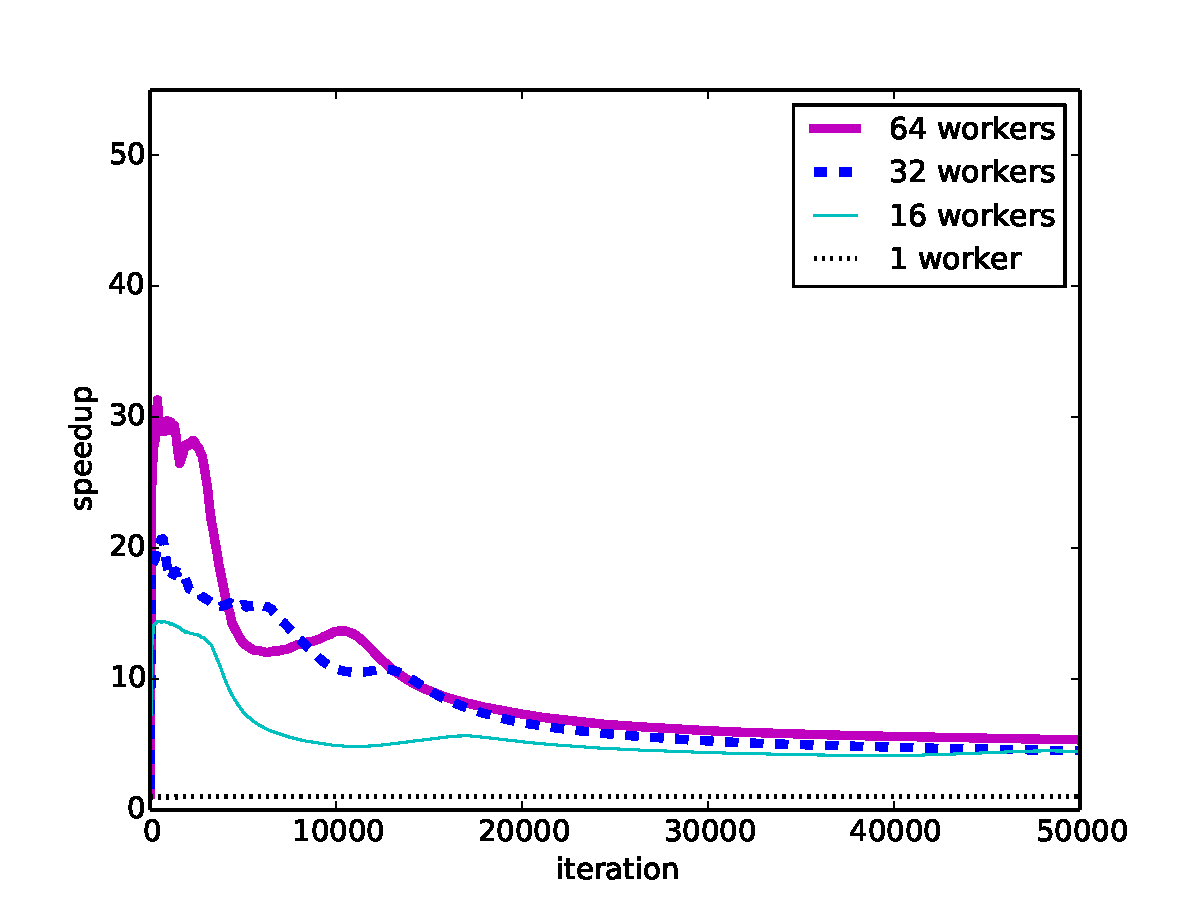
\includegraphics[width=0.65\textwidth]{\fdir/mixture-1-speedup-depth.pdf}
%\includegraphics[width=0.49\textwidth]{figs/mixture-1-speedup-depth-short.pdf}
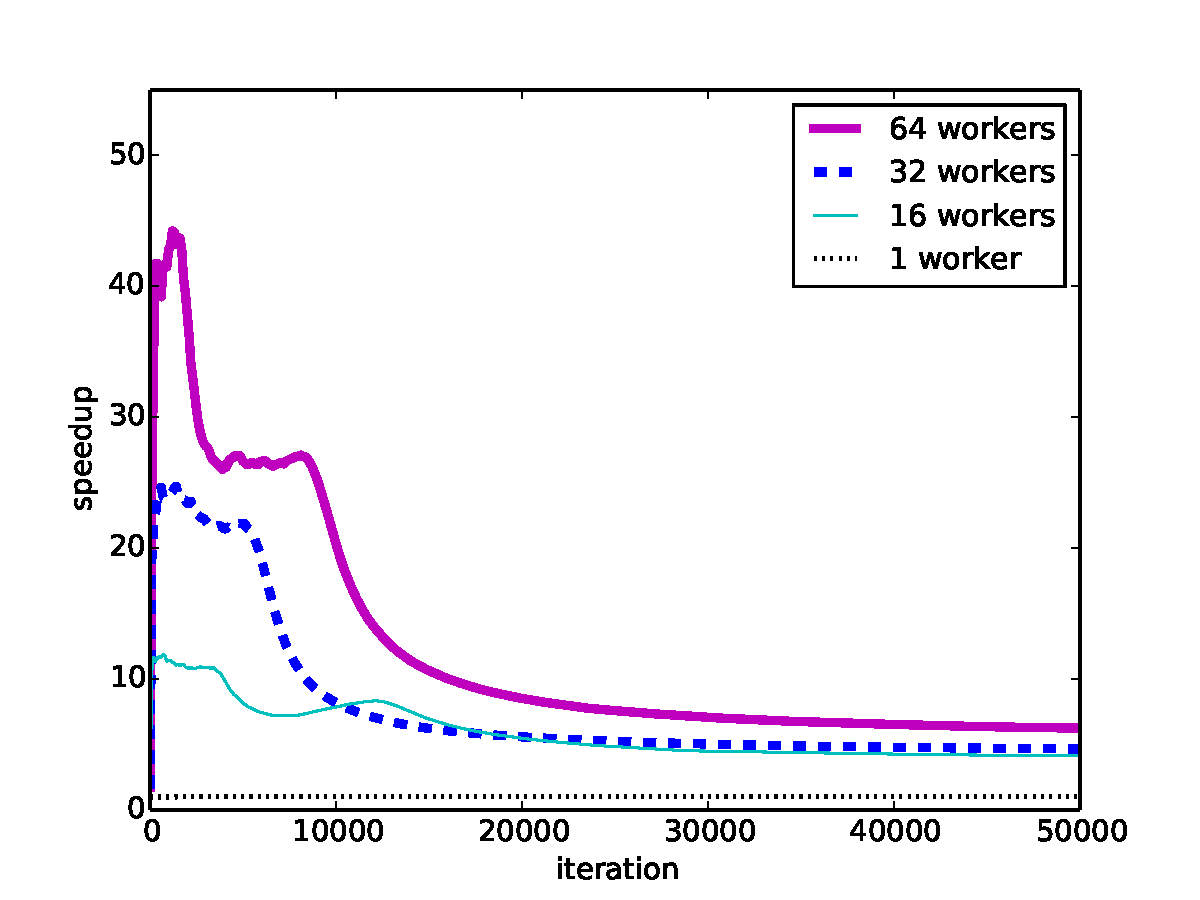
\includegraphics[width=0.65\textwidth]{\fdir/mixture-2-speedup-depth.pdf}
%\includegraphics[width=0.49\textwidth]{figs/thesis-mixture-2-speedup-depth-short.pdf}
\end{center}
\caption{Cumulative speedup relative to our baseline,
as a function of the number of MH iterations, for the mixture of Gaussians problem.
The two figures correspond to different initial conditions,
and the different curves correspond to different numbers of workers.
Pale blue shading highlights the burn-in phase, \ie~the first~${i_1 = 9575}$ iterations.}
\label{fig:mixture}
\end{figure}


Table~\ref{tab:gauss} shows the results for the Gaussian mixture model.
%
We run the model with the same initial conditions and pseudorandom sequences with varying numbers of worker threads. All experiments produce identical chains.
%
We evaluate the cumulative time and speedup obtained at three different iteration counts.
%
The first, ${i_1 = 9575}$ iterations, is burn-in. After $i_1$ iterations, all dimensions of samples achieve the Gelman-Rubin statistic ${\hat R < 1.05}$, computed using two independent chains, where the first $i_1/2$ samples have been discarded~\citep{gelman:1992-inference}.
%
We then run the model further to $i_3$ iterations. Iterations ${i_2 = 24000}$ through ${i_3 = 50000}$ are used to compute an effective number of samples $n_\text{eff}$. (Table~\ref{tab:convergence} shows convergence statistics after $i_3$ iterations.)
%
The results are as we hoped. The initial burn-in phase obtains better-than-logarithmic speedup (though not perfect linear speedup).  With 64 workers, the chain achieves burn-in 16.8$\times$ faster than with one worker.
%
After burn-in, efficiency drops as expected, but we still achieve logarithmic speedup (rather than sub-logarithmic). At $50000$ iterations, speedup for each number of workers $J$ rounds to $\log_2 J$.



\begin{figure}[t!]
\begin{center}
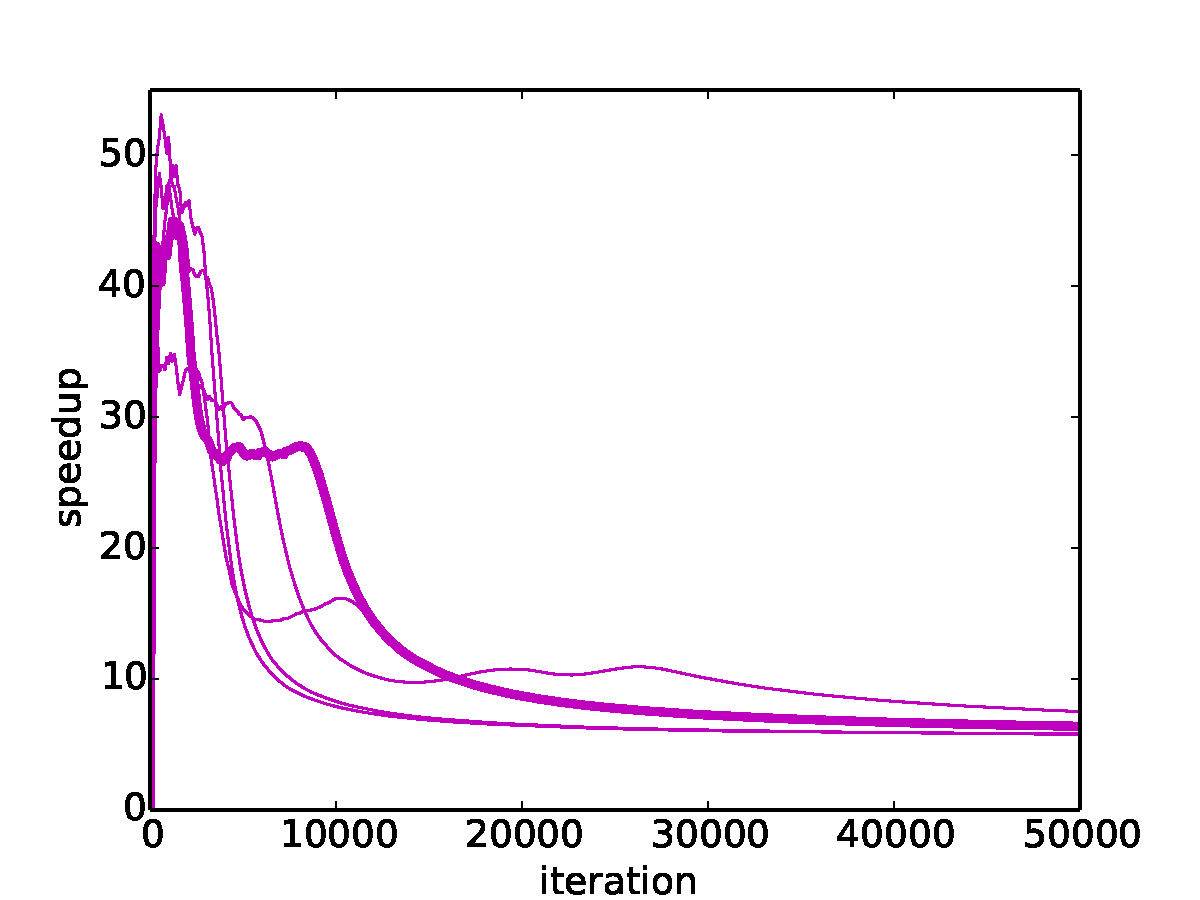
\includegraphics[width=0.65\textwidth]{\fdir/mixture-many-speedup-depth.pdf}
\end{center}
\caption{Cumulative speedup relative to our baseline,
as a function of the number of MH iterations, for the mixture of Gaussians problem.
The different curves correspond to different initial conditions;
all curves are for 64 workers.
Pale blue shading highlights the burn-in phase, \ie~the first~${i_1 = 9575}$ iterations.}
\label{fig:initcond}
\end{figure}

Figure~\ref{fig:mixture} explains these results by graphing cumulative speedup over the whole range of iterations.
%
The initial speedup is good -- we briefly achieve more than~$30\times$ or~$40\times$ speedup, depending on the initial condition, at ${J = 64}$ workers.
%
As burn-in proceeds, cumulative speedup falls off to logarithmic in $J$.
%
Figure~\ref{fig:initcond} shows cumulative speedup for the Gaussian mixture model with several different initial conditions.
%
Each initial condition is drawn from the same generative model as the model parameters, as described in Section~\ref{sec:mixture}.
%
We see a range of variation due to differences in the adaptive scheme during burn-in.
%
The overall pattern is stable, however: good speedup during burn-in followed by logarithmic speedup later.
%
Also note that speedup does not necessarily decrease steadily, or even monotonically. At some initial conditions, the chain enters an easier-to-predict region before truly burning in; while in such a region, speedup is maintained. Our system takes advantage of these regions effectively.

\begin{figure}[t!]
\centering
\vspace{-0.3in}
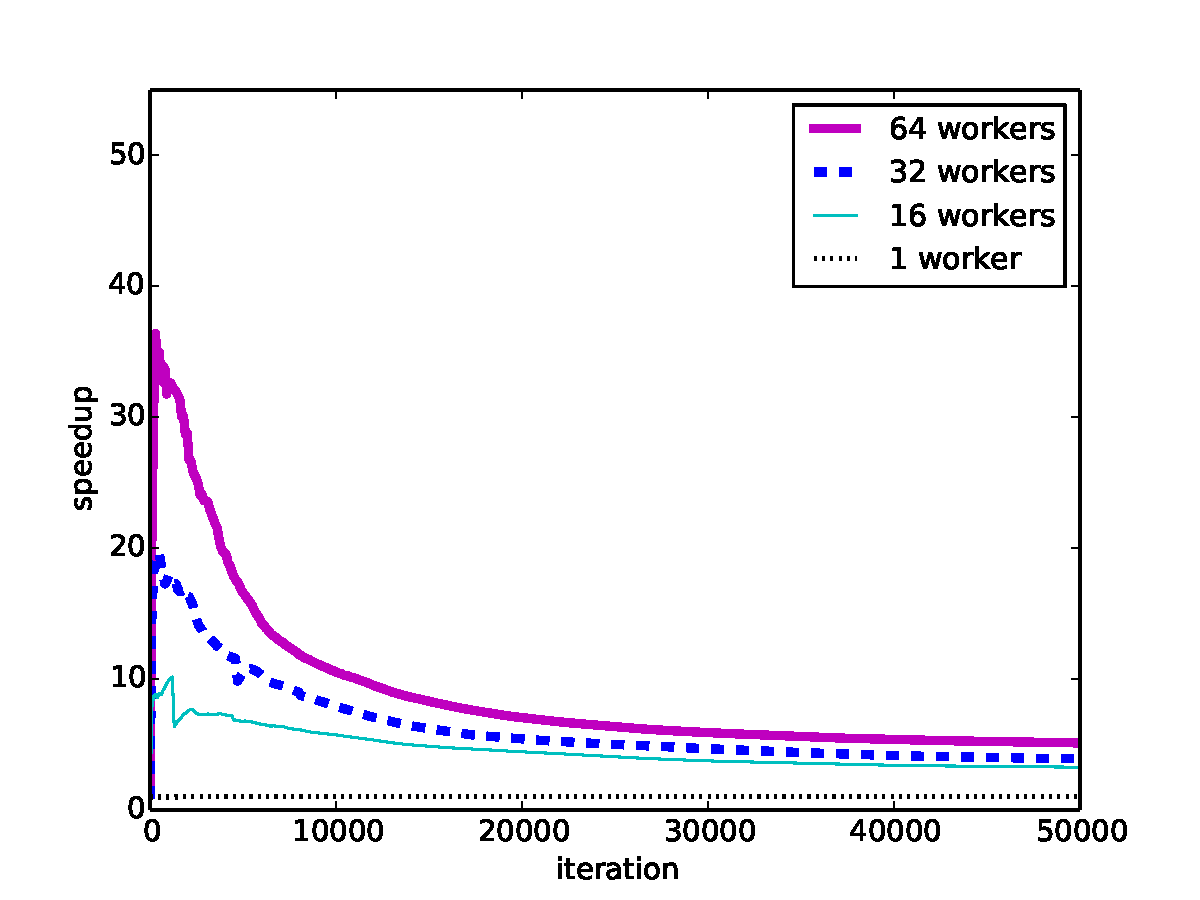
\includegraphics[width=0.56\textwidth]{figs/blasso/blasso-0_1-speedup-depth.pdf}
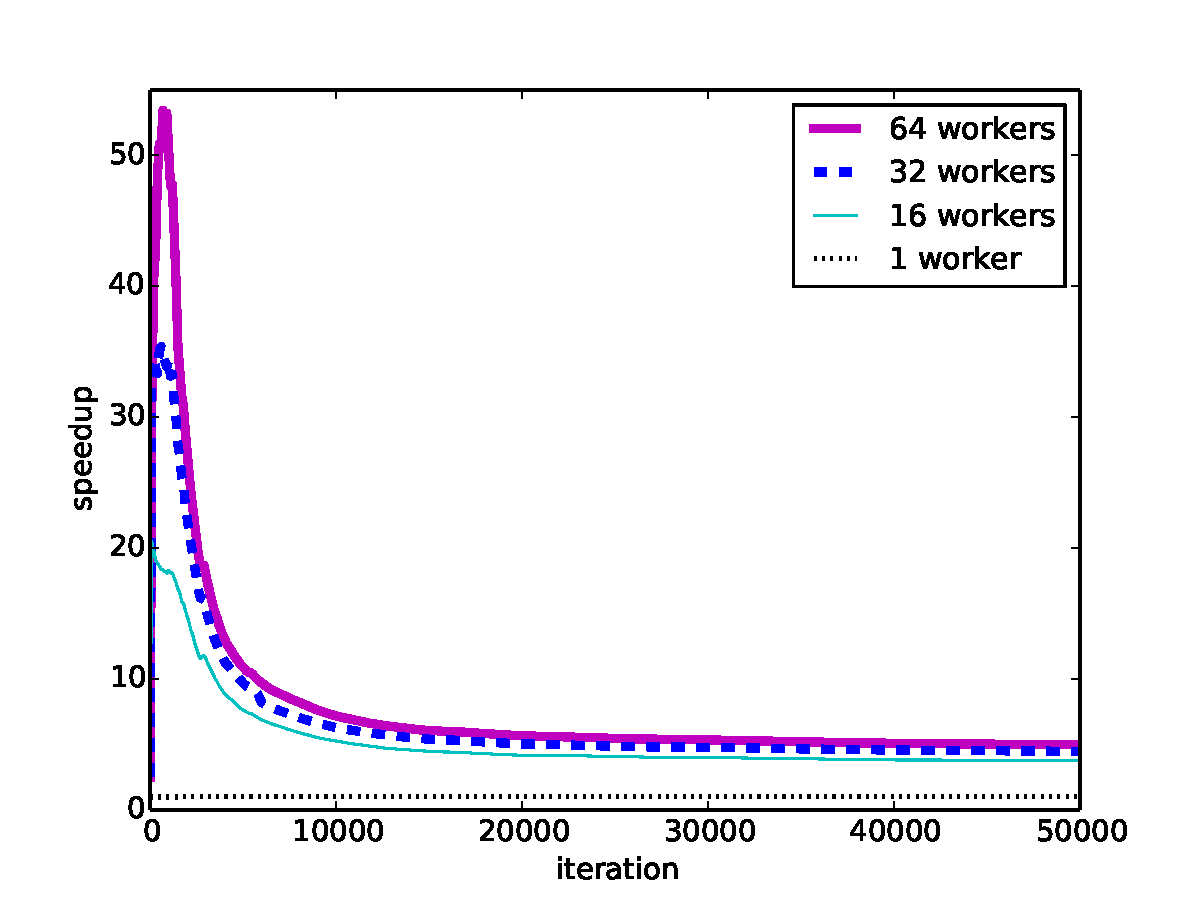
\includegraphics[width=0.56\textwidth]{figs/blasso/blasso-0_01-speedup-depth.pdf}
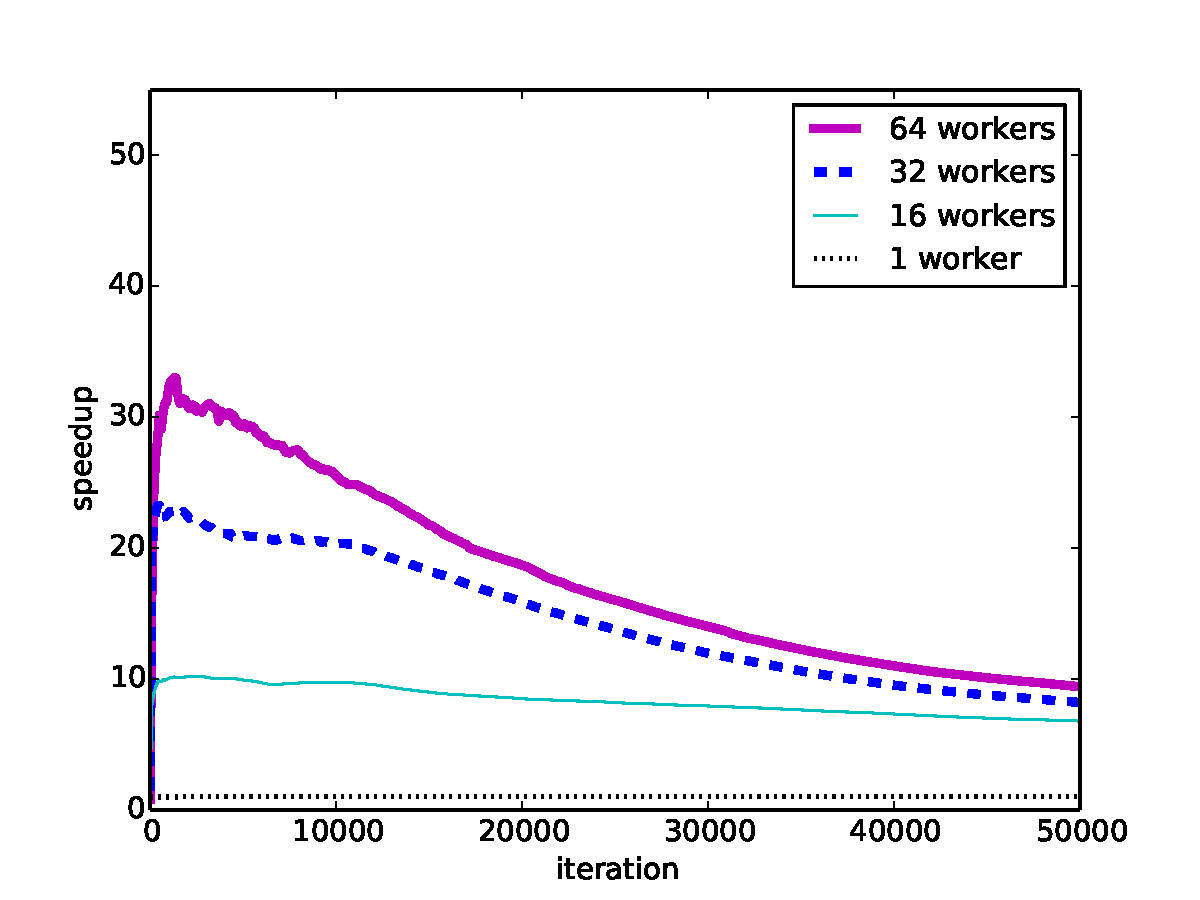
\includegraphics[width=0.56\textwidth]{figs/blasso/blasso-0_1-2-speedup-depth.pdf}
\caption{Cumulative speedup relative to our baseline,
as a function of the number of MH iterations, for the Bayesian Lasso problem.
The different curves correspond to different numbers of workers.
The different figures are for different initial conditions.}
\label{fig:lasso}
\end{figure}

Figure~\ref{fig:lasso} shows that good speedups are achievable for real problems.
%
The speedup behavior for the Bayesian Lasso problem appears similar to that of the mixture of Gaussians.
%
There are differences, however: Lasso evaluation did not converge by 50000 iterations according to standard convergence statistics. On several initial conditions, the chain started taking small steps, and therefore dropped to logarithmic speedup, before achieving convergence.
%
Overall performance might be improved by detecting this case and switching some speculative resources over to other initial conditions, an idea we leave for future work.

\newpage

\section{Adaptive Metropolis--Hastings behavior}

Figure~\ref{fig:adaptive} illustrates the behavior of our adaptive
Metropolis--Hastings algorithm for the mixture of Gaussians problem.
This procedure, described in Section~\ref{sec:adaptive}, adaptively tunes
the proposal distribution to achieve an acceptance rate of~$0.234$.
Specifically, it tunes~${\ell = \log \lambda^2}$, where~$\lambda$ is the scale
of the spherical Gaussian proposal distribution.
Note that the adaptation is not affected by prefetching.
%
Figure~\ref{fig:local-accept-rate} plots a trace of the local acceptance rate,
which we defined in Section~\ref{sec:execution} to be the empirical acceptance
rate observed during the simulation of the~$k$ most recent MH samples.
In our experiments,~${k = \min\{t, 100\}}$, where~$t$ is total number of
MH~samples obtained thus far.
During burn-in, the local acceptance rate varies broadly,
nearly over the entire range of~${[0.0, 0.5]}$,
and afterward settles around the target value of~$0.234$.
Recall that we define burn-in as the first~${i_1 = 9575}$ iterations,
as described in Section~\ref{sec:results} and reported in Table~\ref{tab:gauss}.
%
Figure~\ref{fig:scale} plots the trajectory of the adapted parameter.
As expected, the values of~$\ell$ are larger during burn-in --
when proposals can be made father away without suffering from rejection --
than afterward.
From its initial value,~$\ell$ generally decreases during burn-in, though not
monotonically, until it stabilizes to a small value after convergence.

\begin{figure}[t!]
\centering
%
\vskip\baselineskip
\begin{subfigure}{\textwidth}
\centering
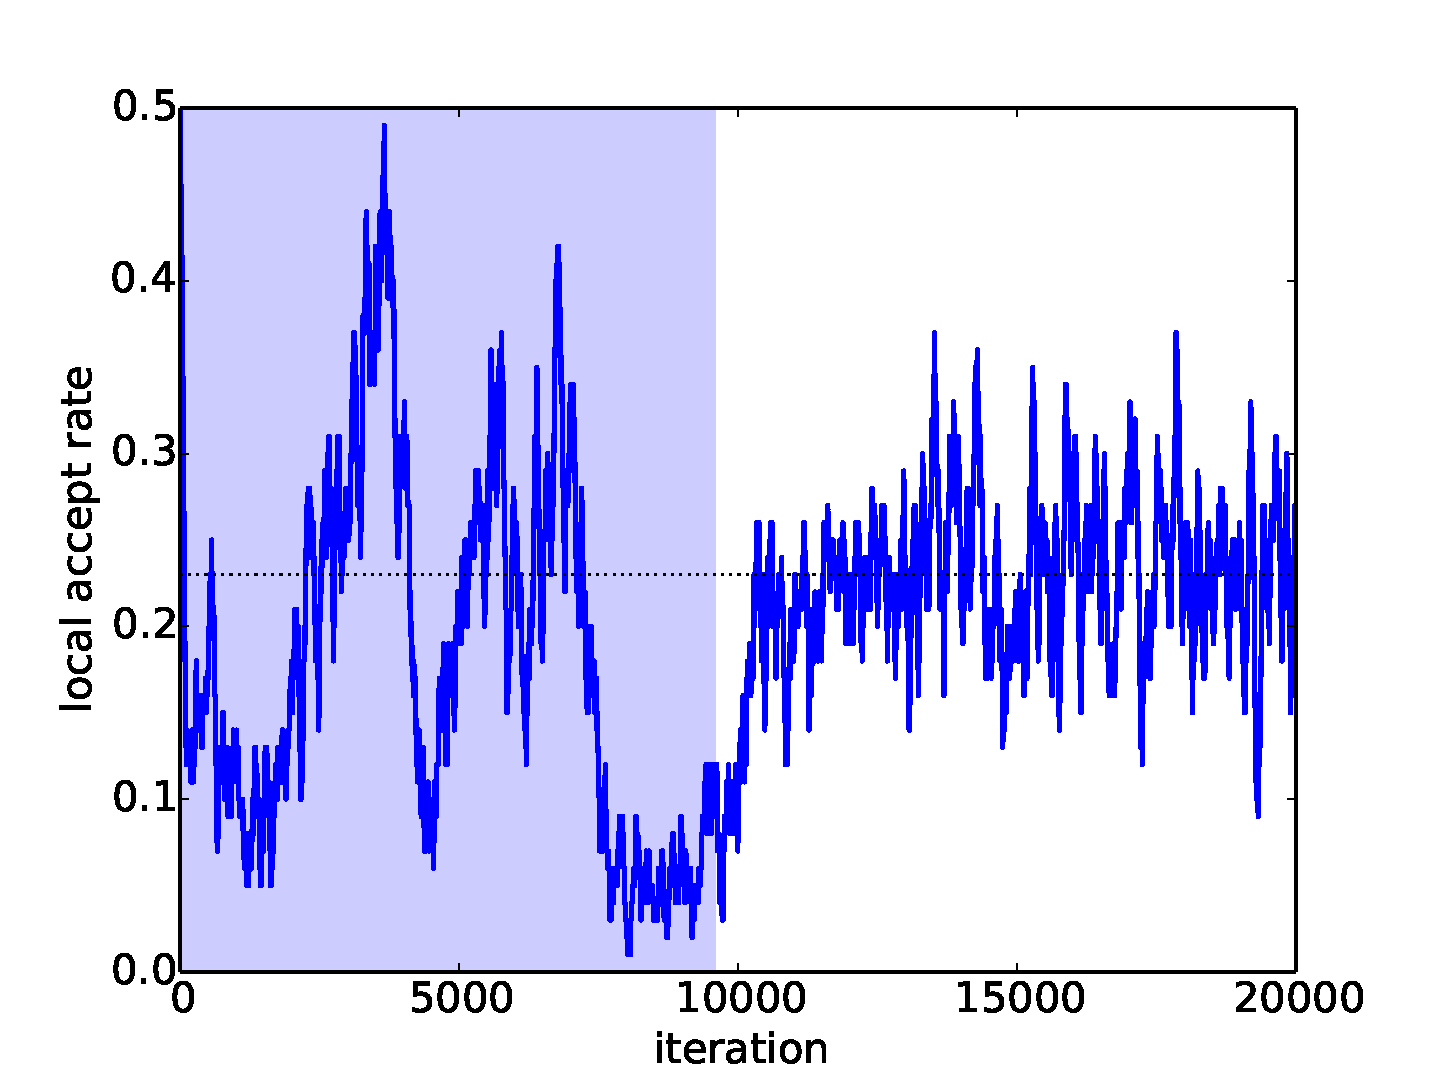
\includegraphics[width=0.65\textwidth]{\fdir/local_accept_rate.pdf}
\vskip.5\baselineskip
\caption{Adaptation during execution of the local acceptance rate.}
\label{fig:local-accept-rate}
\end{subfigure}
\vskip2\baselineskip
\begin{subfigure}{\textwidth}
\centering
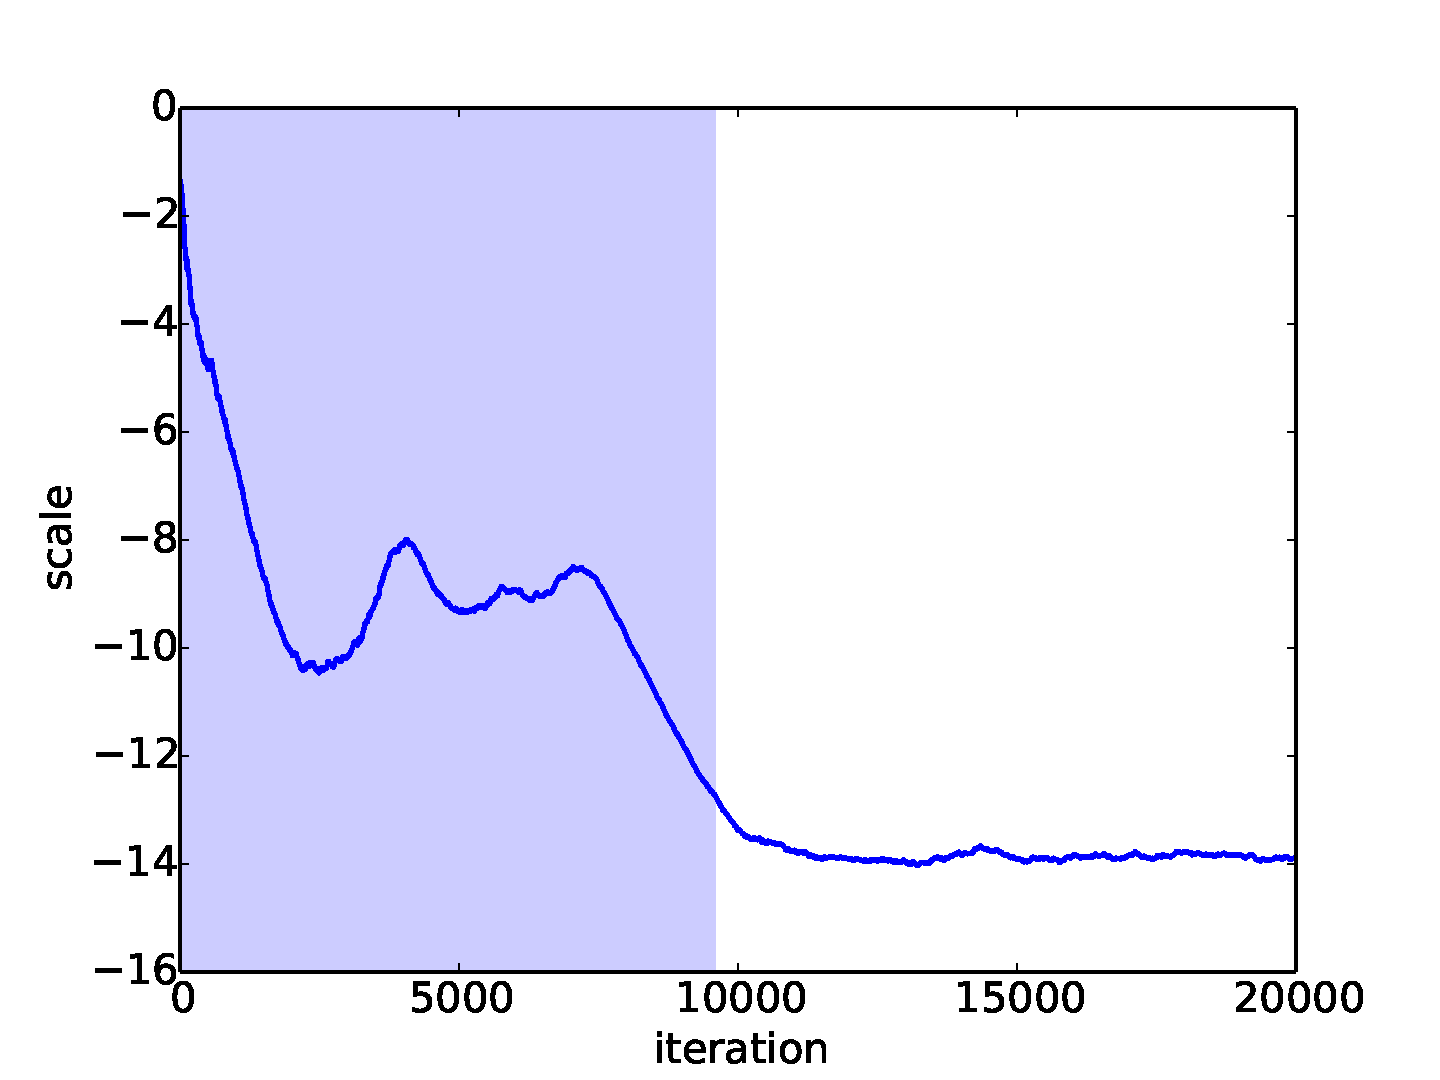
\includegraphics[width=0.65\textwidth]{\fdir/scale.pdf}
\vskip.5\baselineskip
\caption{Adaptation during execution of the proposal distribution's
scale parameter,~$\ell = \log \lambda^2$.}
\label{fig:scale}
\end{subfigure}
%
\caption{Behavior of our adaptive Metropolis--Hastings algorithm, which 
(a)~achieves the target acceptance rate of~$0.234$ by
(b)~tuning the proposal distribution.
Pale blue shading highlights the burn-in phase,
after which the local acceptance rate settles around the target value
and the proposal scale parameter stabilizes.}
\label{fig:adaptive}
\end{figure}

\newpage


\begin{figure}[h!]
\centering
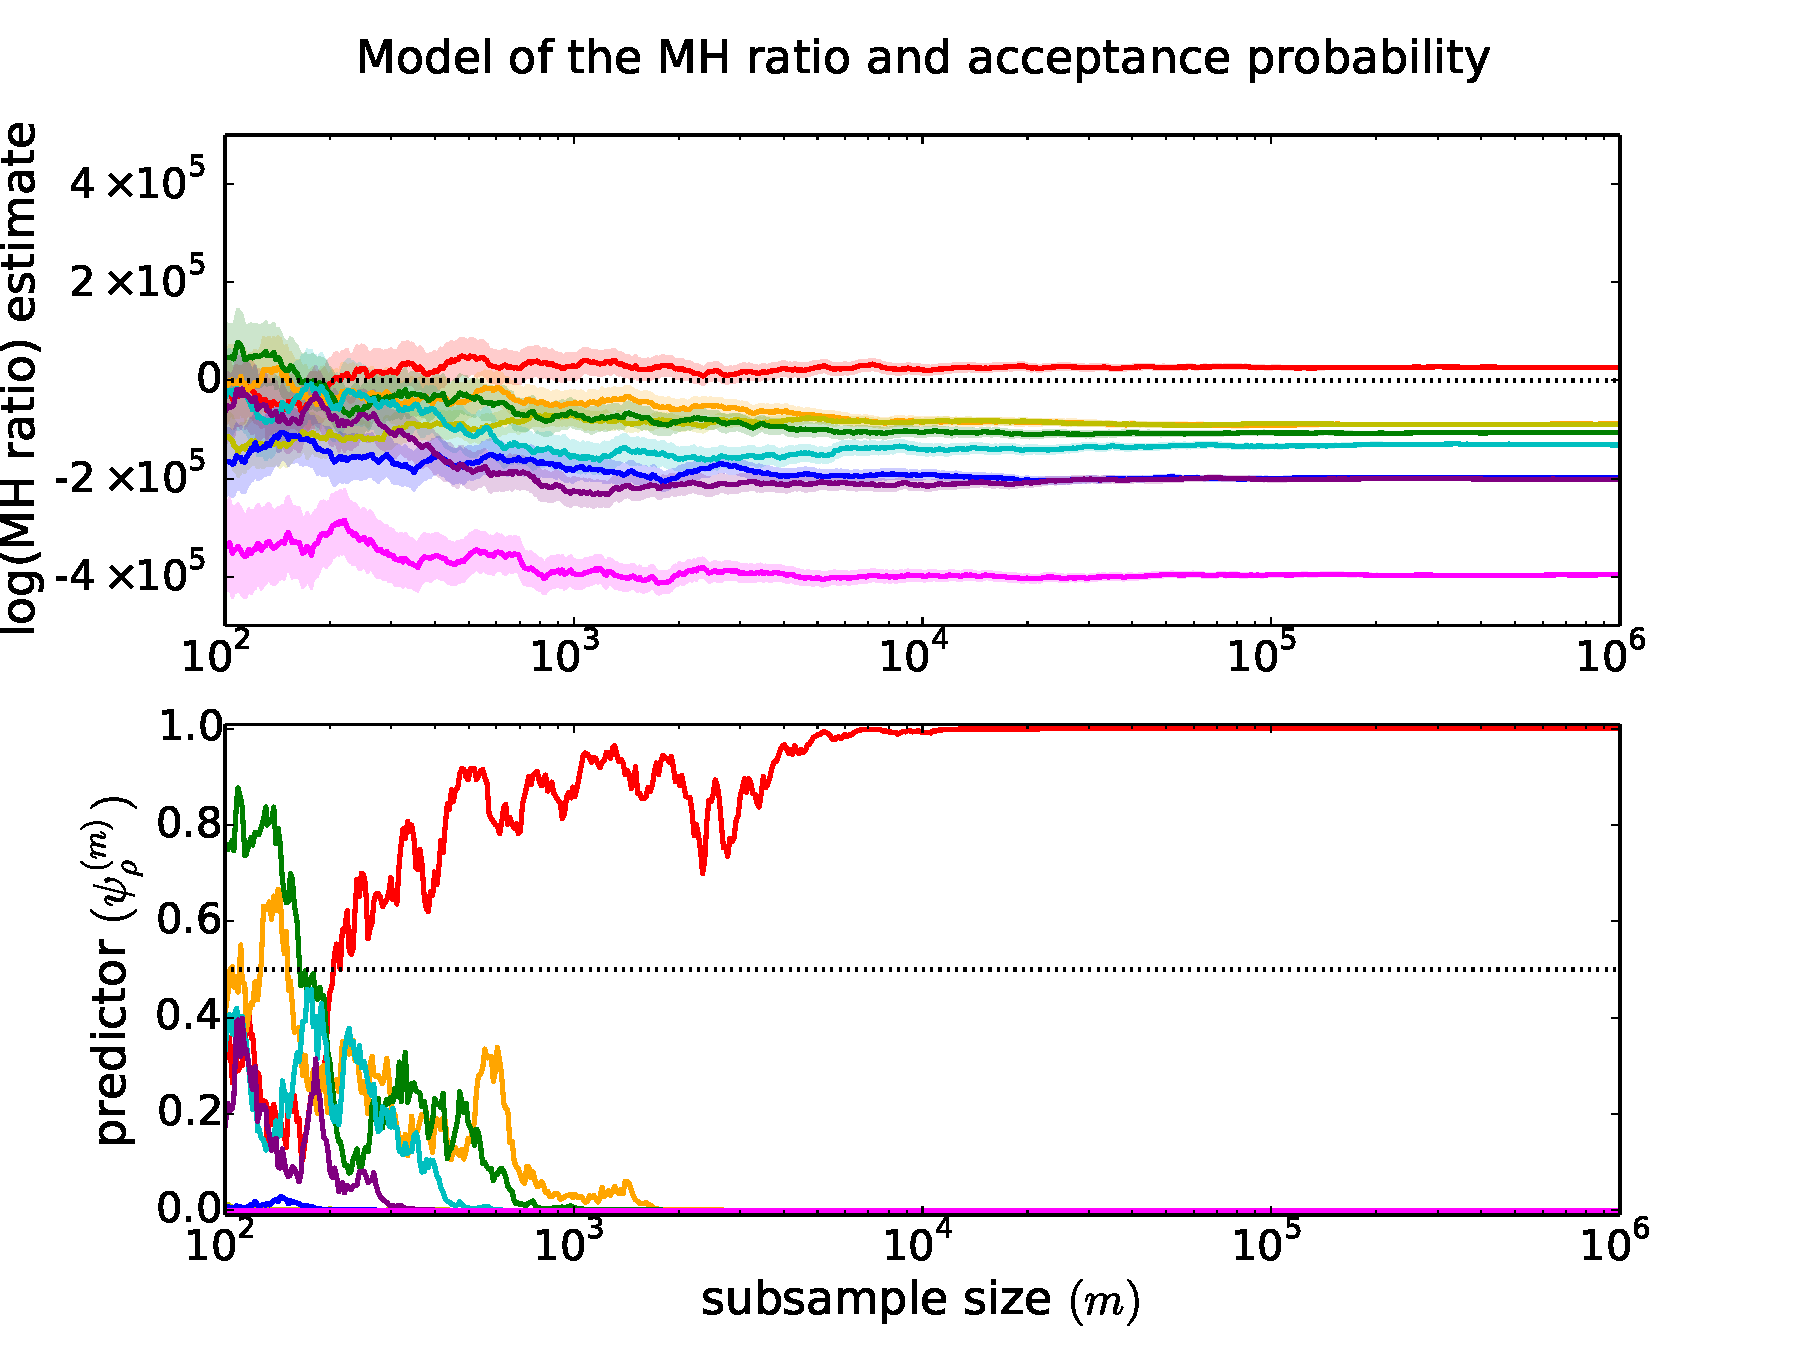
\includegraphics[width=\textwidth]{figs/mix-ic-traces.pdf}
\caption{Example predictor trajectories for the mixture of Gaussians problem
during burn-in.
The upper subfigure plots the estimate of log of the MH ratio
as a function of subsample size~$m$.
The shaded region around each trace indicates one standard deviation in our error model.
The lower subfigure plots the predictor~$\PredEst{\rho}{m}$ as a function of~$m$.
Different colors indicate different~$(\theta, \theta')$ pairs.
Each set of traces corresponds to a sequence of MH iterations.}
\label{fig:ic}
\end{figure}

\begin{figure}[h!]
\centering
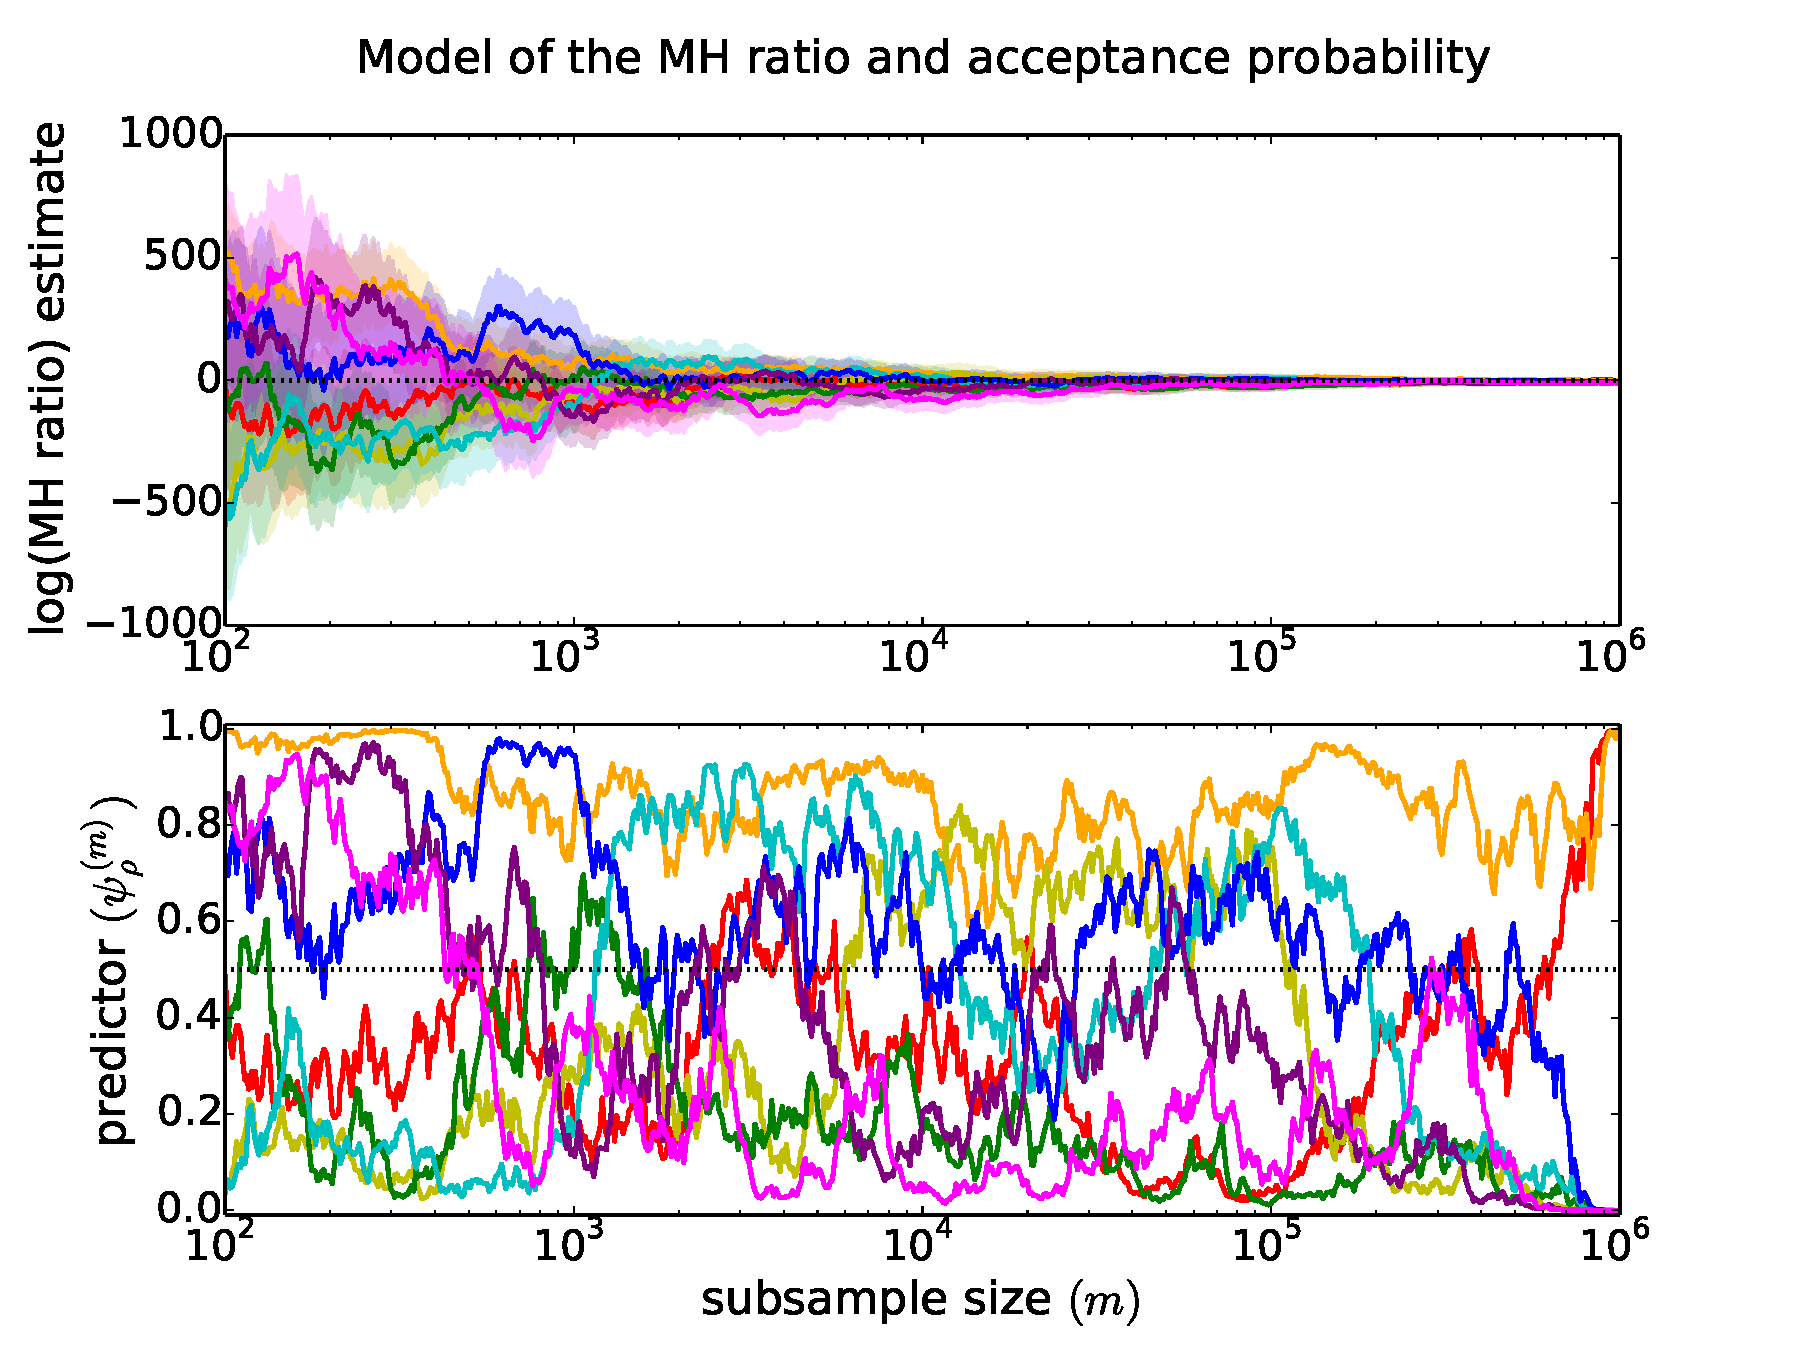
\includegraphics[width=\textwidth]{figs/mix-mle-traces.pdf}
\caption{Example predictor trajectories for the mixture of Gaussians problem
after burn-in.
The upper subfigure plots the estimate of log of the MH ratio
as a function of subsample size~$m$.
The shaded region around each trace indicates one standard deviation in our error model.
The lower subfigure plots the predictor~$\PredEst{\rho}{m}$ as a function of~$m$.
Different colors indicate different~$(\theta, \theta')$ pairs.
Each set of traces corresponds to a sequence of MH iterations.}
\label{fig:mle}
\end{figure}

\section{Estimate, error model and predictor behavior}
\label{sec:predictor-behavior}

In this section, we describe the behavior of our predictor
for the mixture of Gaussians problem.
The predictor depends on the estimate for the log of the Metropolis--Hastings
ratio, the normal error model for this estimate and a uniform random variate~$u$.
Figures~\ref{fig:ic} and~\ref{fig:mle} show the behavior of the estimate,
its error and the subsequent predictors (for randomly chosen~$u$)
during and after burn-in, respectively.
%
At the beginning of burn-in, estimates are effective, and the predictor
converges quite quickly to the correct (final) indicator.
After burn-in, the new proposal's target density is close to the old proposal's,
and the estimates are similarly hard to distinguish.
%
Notice that the scale of the log of their ratio is orders of magnitude smaller
after burn-in compared to the beginning of burn-in.
The random variate~$u$ could be small enough for the predictor to
converge quickly to 1; more often, the predictor varies widely over time,
and does not converge to~$0$ or~$1$ until almost all data are evaluated.
This behavior makes logarithmic speedup a best case.
Luckily, the predictor is more typically uncertain (with an intermediate value)
than wrong (with an extreme value that eventually flips to the opposite value):
incorrect predictors could lead to sublogarithmic speedup.


%\begin{figure}[t!]
%\begin{center}
%\includegraphics[width=0.65\textwidth]{figs/mix-ic-permutations.pdf}
%\end{center}
%\caption{The estimate of the log posterior as a function of subsample size.
%Different colors correspond to different random permutations of the data.
%}
%\label{fig:permutations}
%\end{figure}

\begin{figure}[t!]
\begin{center}
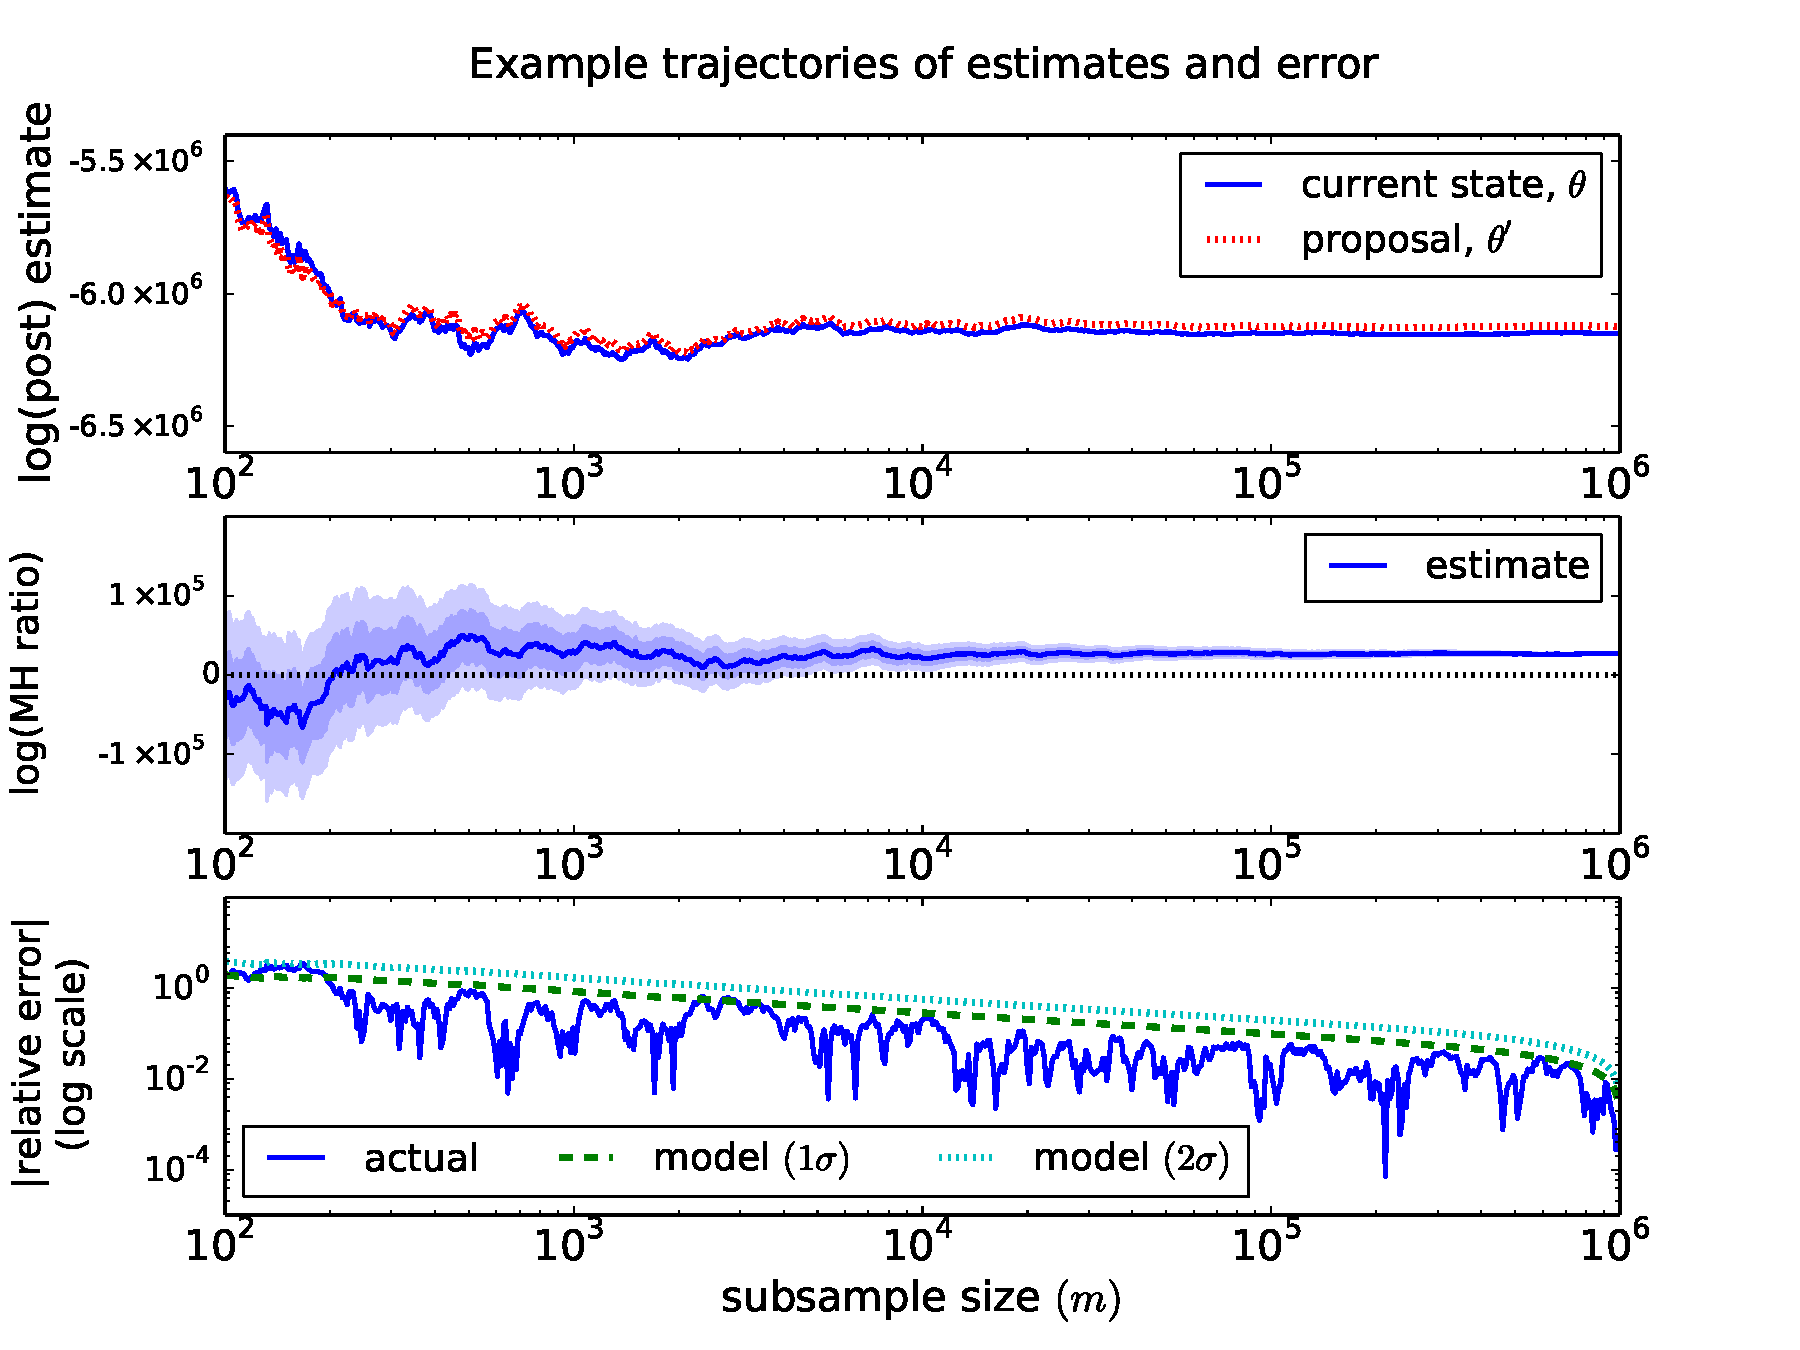
\includegraphics[width=\textwidth]{figs/mix-ic-traces-pair.pdf}
\end{center}
\caption{Estimates and error during burn-in.
Each subfigure plots traces as a function of subsample size.
The upper subfigure plots the estimates of the log posterior at
the current state (solid blue) and proposal (dotted red).
The middle subfigure plots the estimate of the log MH ratio (solid line),
with shaded regions indicating one (dark) and two (light) times the standard error.
The lower subfigure plots on a log scale the absolute error of this estimate
relative to the true (final) value (solid blue),
as well as one (dashed green) and two (dotted cyan) times the standard error.
}
\label{fig:pair-ic}
\end{figure}

Our estimates depend on the order in which the data are evaluated.
%Figure~\ref{fig:permutations} plots multiple trajectories of a single true
%log posterior estimate, for different permutations of the data.
In general, we might be worried about malicious orderings of the data,
which could lead to biased estimates, bad predictors and performance degradation.
In our experiments, we permute the data once at the very beginning.
A more sophisticated solution would be to occasionally re-permute the data
during execution, \eg every~20 iterations or so.
Our current implementation could be modified to support this,
but care would be required to avoid hurting performance.
For example, suppose we decide to permute the data after accepting state~$\theta'$.
At the next iteration, MH compares~$\theta$ to~$\theta'$,
but each is now associated with a different ordering of the data.
This is unfavorable because our predictors work best when the data are
evaluated in the same order for both~$\theta$ and~$\theta'$.

\begin{figure}[t!]
\begin{center}
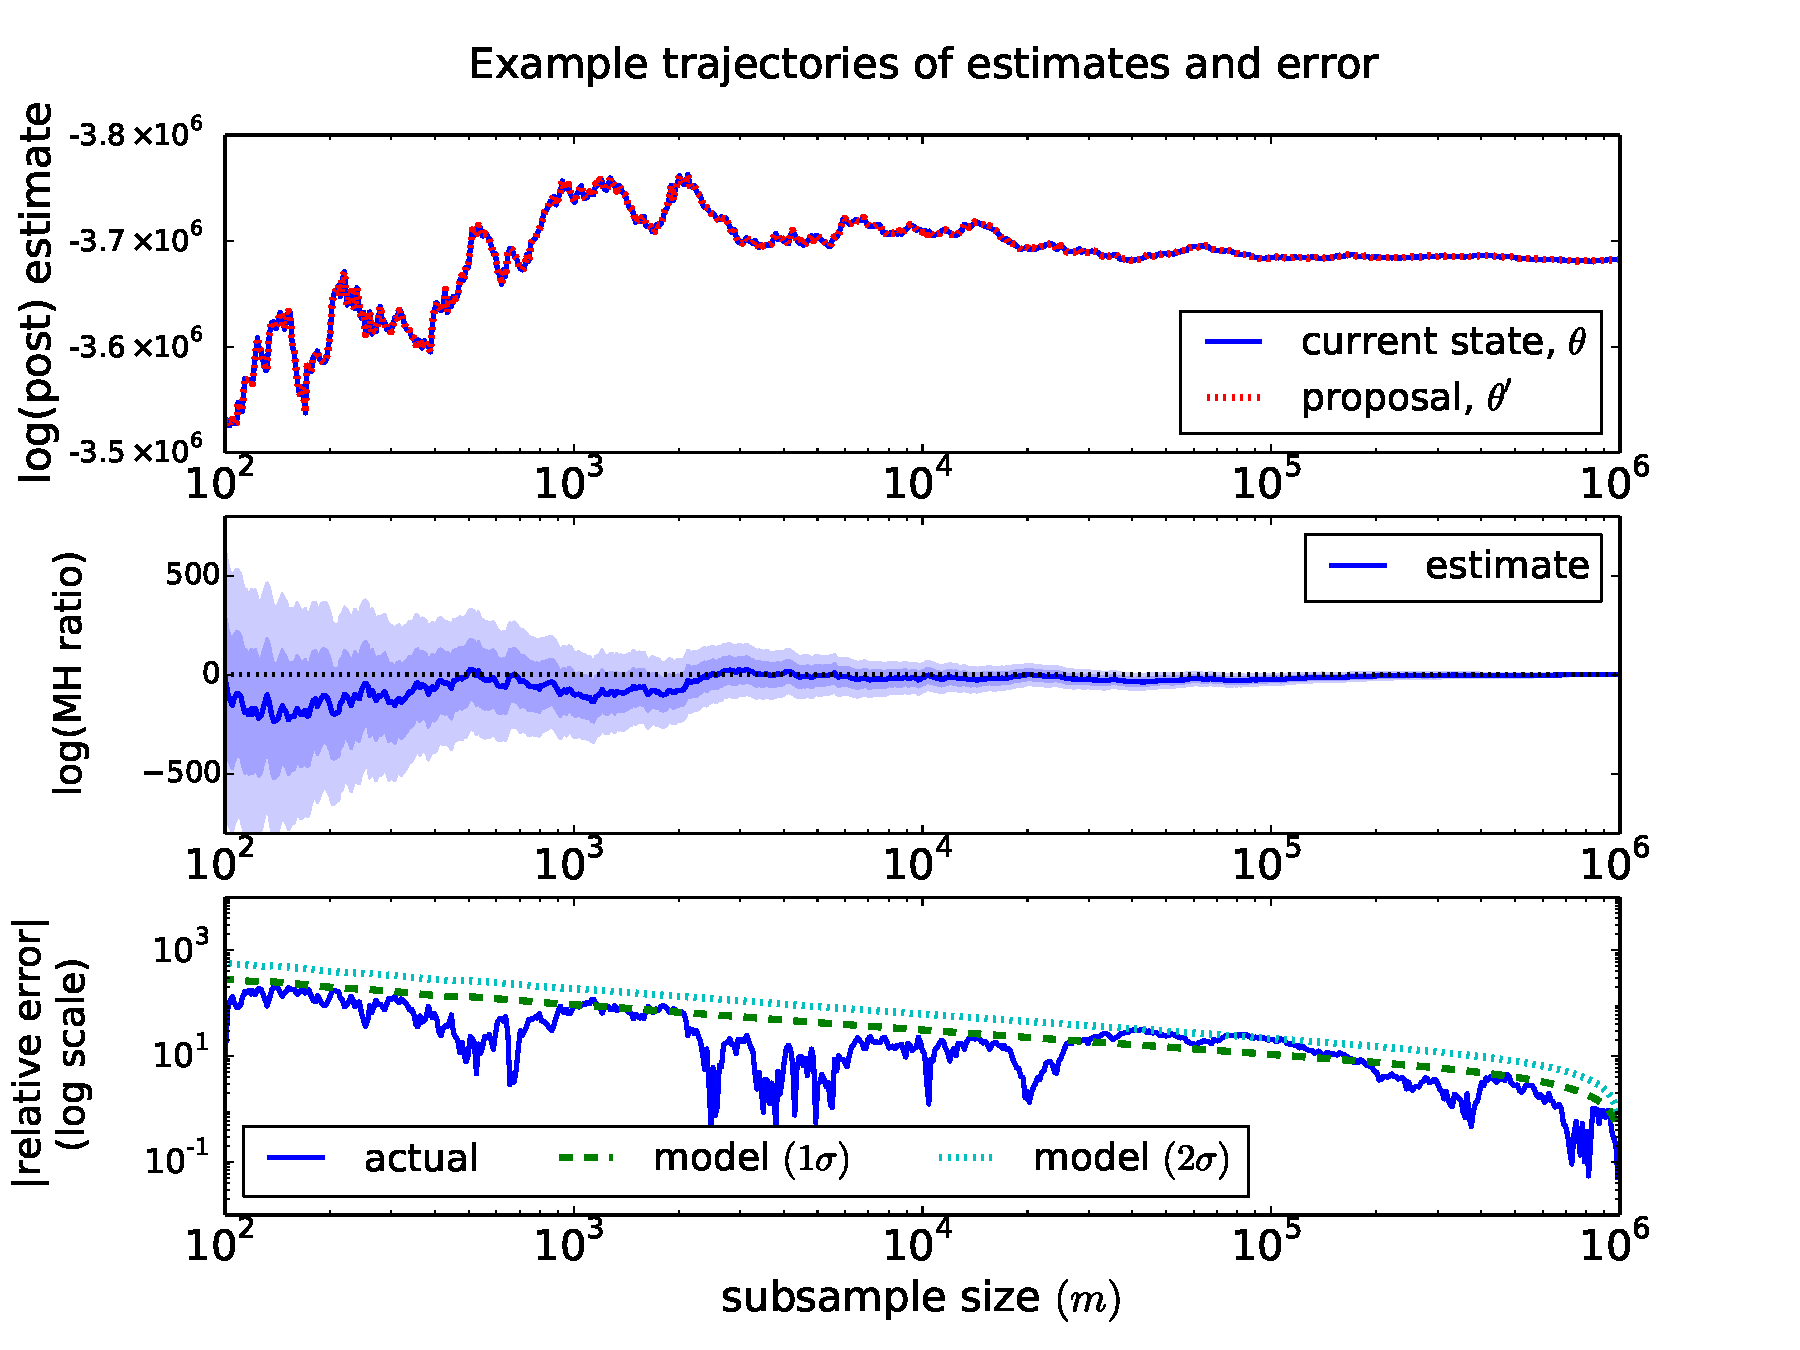
\includegraphics[width=\textwidth]{figs/mix-mle-traces-pair.pdf}
\end{center}
\caption{Estimates and error at convergence, analogous to Figure~\ref{fig:pair-ic}.}
\label{fig:pair-mle}
\end{figure}

Figures~\ref{fig:pair-ic} and~\ref{fig:pair-mle} illustrate, in greater detail,
the evolution of the MH ratio estimate, during and after burn-in, respectively.
%
Each upper subfigure separately plots the estimates of the log posterior at the
current state and the proposal.
These traces are highly correlated, since the log likelihoods at the current
state and proposal are highly correlated for each datum.
At the beginning of burn-in, the correlation between~$\log \pi(\theta \given x_i)$
and~$\log \pi(\theta' \given x_i)$ is greater than~${0.9}$;
after convergence, it is greater than~${0.9999}$.
This summarizes why it becomes more difficult to predict whether a proposal will
be accepted or rejected -- the target evaluations at~$\theta$ and~$\theta'$ are
practically indistinguishable.
%
Each middle subfigure plots the corresponding estimate of the log MH ratio,
which cross the dotted line at zero whenever the above estimates cross.
Shading around the estimate corresponds to our error model.
%
Each lower subfigure plots the error of this estimate relative to the true (final)
value on a log scale; our model is consistent with the actual error.

\begin{figure}[t!]
\begin{center}
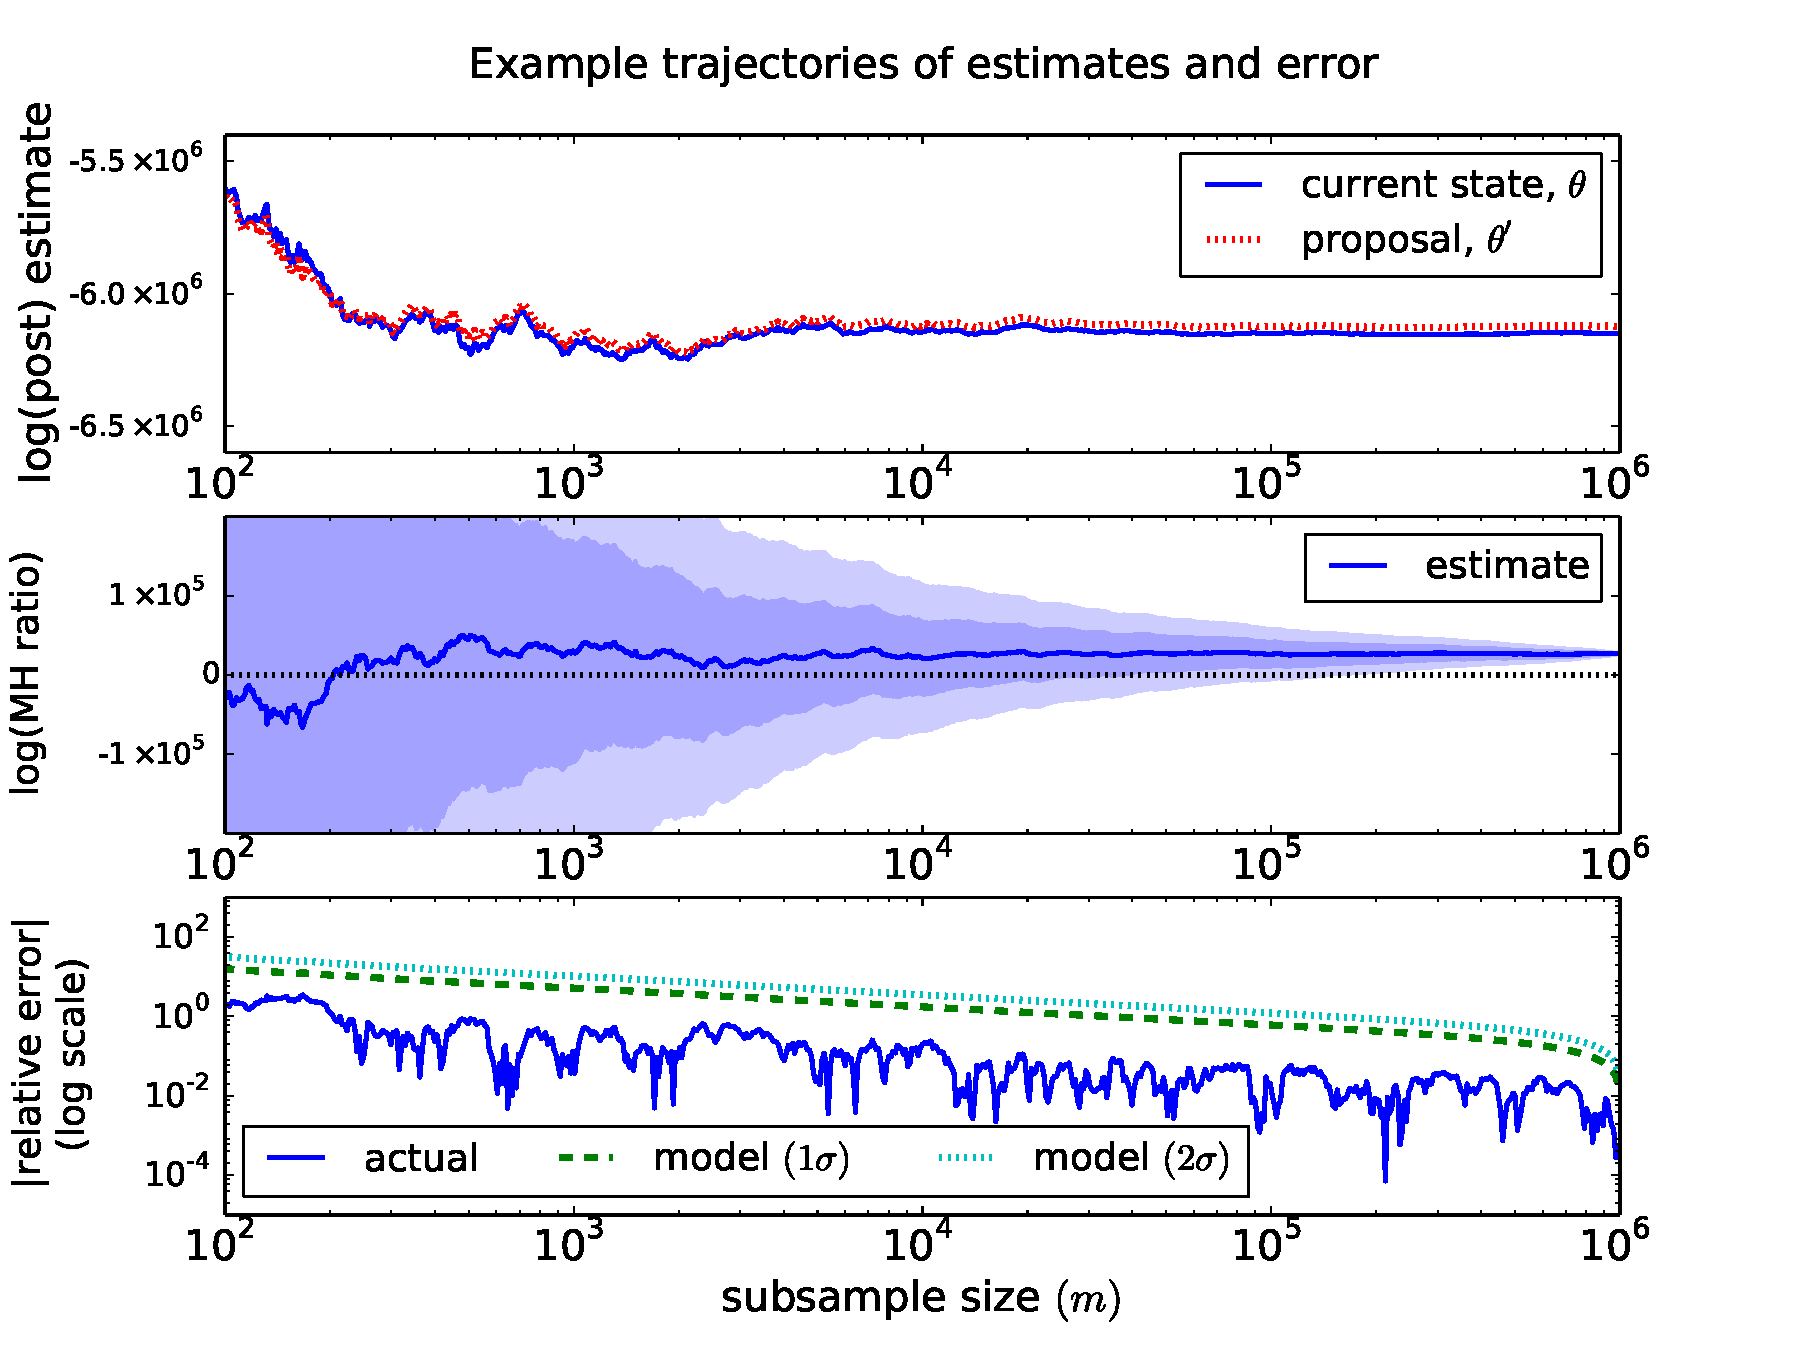
\includegraphics[width=\textwidth]{figs/eddie/mix-ic-traces-pair.pdf}
\end{center}
\caption{Estimates and na\"ive error model during burn-in.
The estimates are the same as in Figure~\ref{fig:pair-ic},
but the error is significantly worse.
Note that the scales of all the axes are the same as those in Figure~\ref{fig:pair-ic}.}
\label{fig:naive-error}
\end{figure} 

\begin{figure}[t!]
\begin{center}
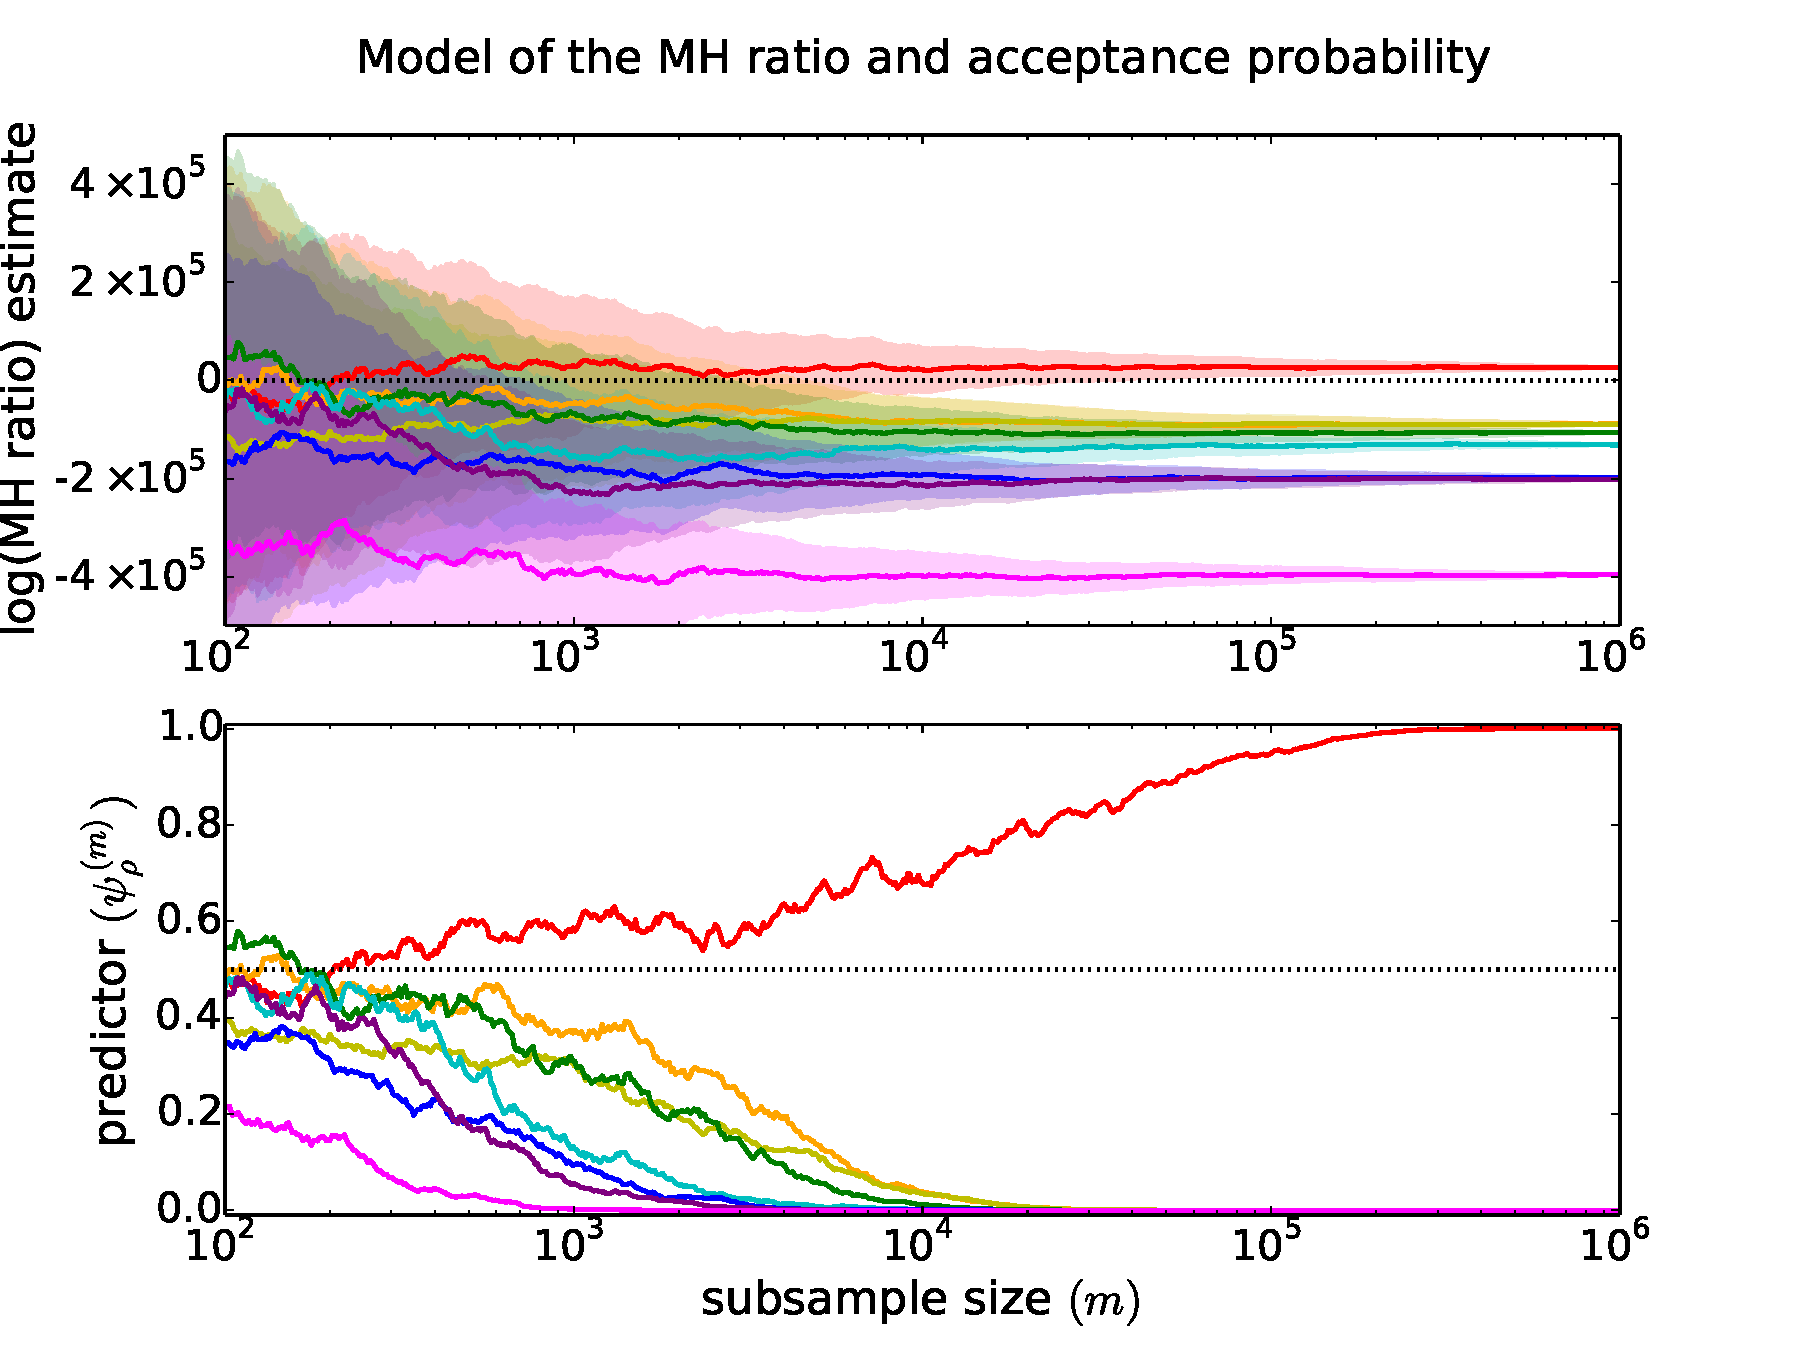
\includegraphics[width=\textwidth]{figs/eddie/mix-ic-traces.pdf}
\end{center}
\caption{Example predictor trajectories for the mixture of Gaussians problem
during burn-in.
The trajectories and estimates are the same as in Figure~\ref{fig:ic},
but here we use the na\"ive error model, as in Figure~\ref{fig:naive-error}.
}
\label{fig:naive-predictor}
\end{figure} 

Our choice of error model has a significant impact on the predictors we form
to make scheduling decisions.
Figure~\ref{fig:naive-error} illustrates a na\"ive approach, briefly mentioned in 
Section~\ref{sec:estimator}, that separately models the estimates for the
log posteriors at~$\theta$ and~$\theta'$ without capturing the correlation
between~$\log \pi(\theta \given x_i)$ and~$\log \pi(\theta' \given x_i)$.
As expected, the estimates for the full log posteriors are the same as before,
but the estimated error is dramatically larger.
This translates to inaccurately high uncertainty in the estimates
and would result in needlessly conservative speculation.
This is illustrated in Figure~\ref{fig:naive-predictor}, which by comparison to
Figure~\ref{fig:ic} shows that the na\"ive error model results in predictors
that must evaluate about an order of magnitude more data to converge.
Note that these examples are representative of the beginning of burn-in;
we expect the predictors to require even more data to converge as the
execution progresses.
Thus with the na\"ive error model, we would expect predictive prefetching to
yield smaller benefits.

To see how predictor behavior changes over the course of execution, we track
two quantities during execution that summarize the trajectory of each predictor
concerned with an accept/reject decision on the true Markov chain path.
%
Figure~\ref{fig:threshold-position} plots the~\emph{threshold position},
which we define as the smallest number of batches evaluated after which the
predictor does not cross~0.5,
\ie one greater than the last batch leading to an incorrect prediction. 
Recall that in our experiments, the total number of batches is~$100$.
The threshold position tends to increase over the course of execution,
with a relatively sharp phase transition from burn-in to convergence.
After convergence, essentially all the data must be inspected.
%
Figure~\ref{fig:flip-count} plots the~\emph{flip count}, which we define as the
number of times the predictor crosses~$0.5$, \ie the number of times it
``changes its mind'' about whether the proposal will be accepted or rejected.
The flip count also tends to increase over the course of execution,
though it doesn't exhibit quite the dramatic transition as the threshold position.
%
Both threshold position and flip count exhibit behavior consistent with
Figures~\ref{fig:ic} and~\ref{fig:mle}.

\begin{figure}[t!]
\centering
%
\begin{subfigure}{\textwidth}
\centering
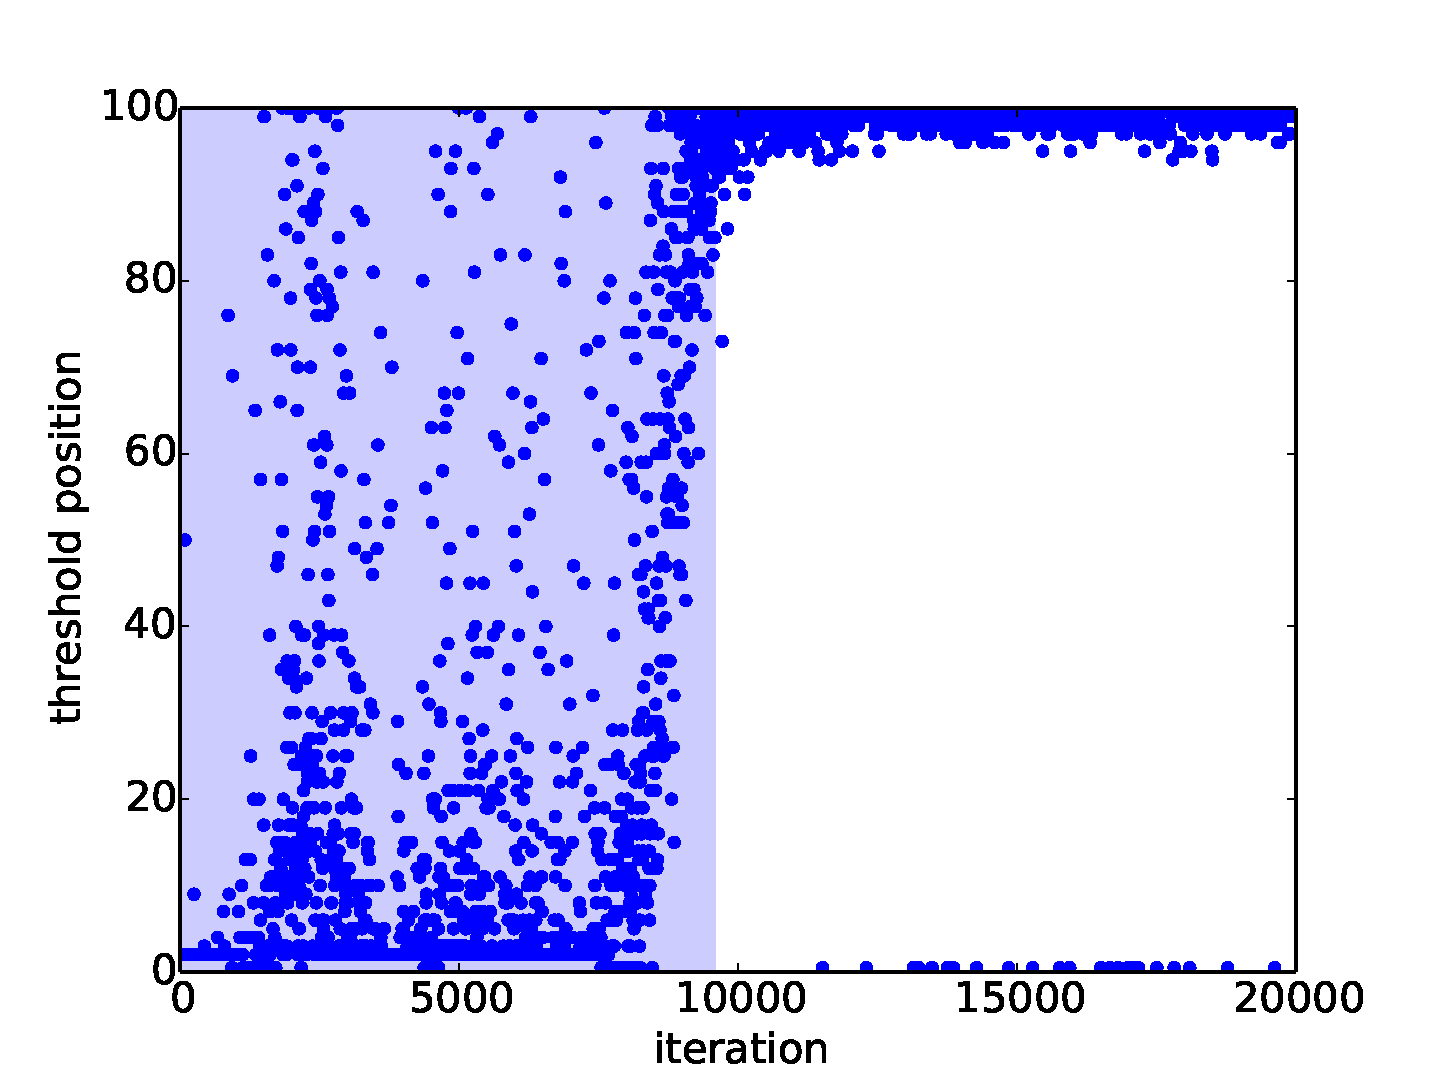
\includegraphics[width=0.65\textwidth]{\fdir/threshold_position.pdf}
\vskip.5\baselineskip
\caption{Threshold position.}
\label{fig:threshold-position}
\end{subfigure}
\vskip1\baselineskip
\begin{subfigure}{\textwidth}
\centering
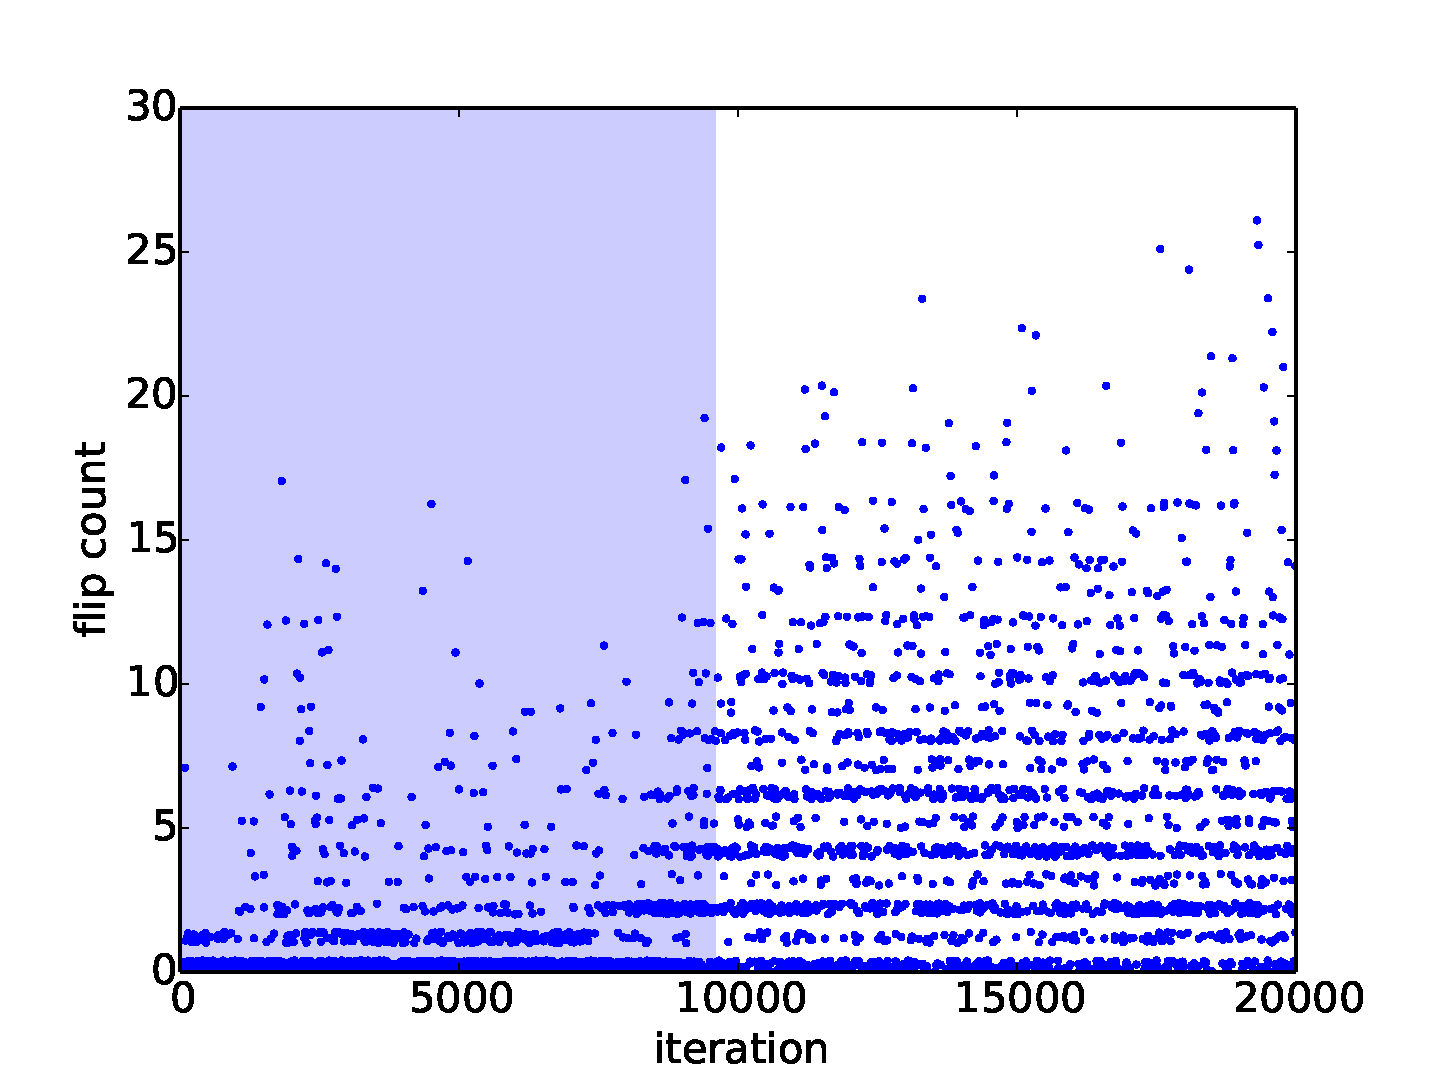
\includegraphics[width=0.65\textwidth]{\fdir/flip_count.pdf}
\vskip.5\baselineskip
\caption{Flip count.}
\label{fig:flip-count}
\end{subfigure}
%
\vskip1\baselineskip
\caption{Summaries of predictor behavior.
Note that the data have been downsampled by a factor of five,
and pale blue shading highlights burn-in.
(a)~The threshold position tends to increase over the course of execution.
(b)~The flip count tends to increase over the course of execution.
For visual clarity, we have added a small amount of jitter, distributed
uniformly and randomly on~${[0, 0.4)}$, to the integer-valued counts.}
\end{figure}


\newpage

\section{System measurements}
\label{sec:measurements}

In the previous section, we presented our main evaluation in terms of speedup.
Here, we explain these results through measurements that characterize our system's behavior.
As expected, we do not achieve perfect speedup, and the dominant reason is that
only some of the speculative computation performed by workers is \emph{useful};
any extra computation is not useful and we call it \emph{wasted}.
Figure~\ref{fig:useful-wasted} illustrates the distribution of useful (blue)
and wasted (light gray) work on the Metropolis--Hastings binary tree,
for a particular simulation path corresponding to the true output (thick arrows).
Ignoring communication and other system overheads, perfect speedup is achieved
when computation is performed only at the useful nodes.
Lower \emph{efficiency} is the result of wasted computation at other nodes
and is given by the fraction of total computational time spent on useful work.
Ideally, efficiency would equal~1, leading to perfect speedup.
In practice, efficiency is less than~1 due to wasted work and other overheads.
The measurements below explain these inefficiencies.
In this section we focus on the mixture of
Gaussians problem with 64 workers, specifically, the experiment using
the second initial condition shown in Figure~\ref{fig:mixture},
with~$N=10^6$ data in the likelihood, evaluated in~100 batches.

\begin{figure}[t!]
  \centering%
  \resizebox{\columnwidth}{!}{%
    \def\radius {8mm}
    \tikzstyle{state}=[circle, thick, inner sep=0pt, minimum size=\radius, font=\footnotesize, draw]
    \tikzstyle{wasted}=[circle, thick, fill=LightGray, inner sep=0pt, minimum size=\radius, font=\footnotesize, draw]
    \tikzstyle{useful}=[circle, thick, fill=CornflowerBlue, inner sep=0pt, minimum size=\radius, font=\footnotesize, draw]
    \begin{tikzpicture}[->,>=stealth',level/.style={sibling distance = 5.5cm/#1, level distance = 1.5cm}]
      \draw [white,-] (-6cm,-0.75cm) -- (6cm,-0.75cm);
   %   \draw [gray,-] (-6cm,-2.25cm) -- (6cm,-2.25cm);
   %   \draw [gray,-] (-6cm,-3.75cm) -- (6cm,-3.75cm);
      \node [useful] (root) {$x^t_\emptystr$}
      child{ node [state] {$x^{t+1}_\bits{0}$}
        child{ node [state] {$x^{t+2}_\bits{00}$}
          child{ node [state] {$x^{t+3}_\bits{000}$}}
          child{ node [wasted] {$x^{t+3}_\bits{001}$}}
        }
        child{ node [wasted] {$x^{t+2}_\bits{01}$}
          child{ node [state] {$x^{t+3}_\bits{010}$}}
          child{ node [wasted] {$x^{t+3}_\bits{011}$}}
        }
      }
      child{ node [useful] {$x^{t+1}_\bits{1}$}
        child{ node [state] {$x^{t+2}_\bits{10}$}
          child{ node [state] {$x^{t+3}_\bits{100}$}}
          child{ node [useful] {$x^{t+3}_\bits{101}$}}
        }
        child{ node [useful] {$x^{t+2}_\bits{11}$}
          child{ node [state] {$x^{t+3}_\bits{110}$}}
          child{ node [wasted] {$x^{t+3}_\bits{111}$}}
        }
      }
      ;
   %   \node [state] at (5.5cm, 0) {$\uu^{t}$};
   %   \node [state] at (5.5cm, -1.5) {$\uu^{t+1}$};
   %   \node [state] at (5.5cm, -3) {$\uu^{t+2}$};
   %   \node [state] at (5.5cm, -4.5) {$\uu^{t+3}$};
      \draw [->, ultra thick, Dandelion] (root) to (root-2);
      \draw [->, ultra thick, Dandelion] (root-2) to (root-2-1);
      \draw [->, ultra thick, Dandelion] (root-2-1) to (root-2-1-1);
    \end{tikzpicture}
  }
  \caption{Metropolis--Hastings binary tree.
  Suppose that the thick arrows connect samples output by the algorithm.
  The blue circles then highlight nodes where computation must be performed,
  corresponding to useful work.
  When a prefetching scheme performs computation at the light gray nodes,
  this wasted work does not advance computation.
  Each remaining node is a copy of its parent and thus does not demand new computation.}
  \label{fig:useful-wasted}
\end{figure}


During execution, our system exhibits different phases of behavior.
Figure~\ref{fig:progress} plots overall progress as a function of wall clock time.
There are two main phases: during and after burn-in.
Progress is roughly constant within each phase
and at least three times faster during burn-in than afterward;
at least the first~10\% of burn-in is even faster.
From this trace, we choose iteration counts representative of these three phases:
500, 5000 and 15000.
Below, we present a decomposition of how computational resources are utilized,
at each of these iteration counts, on both the workers and the master.


\begin{figure}[t!]
\begin{center}
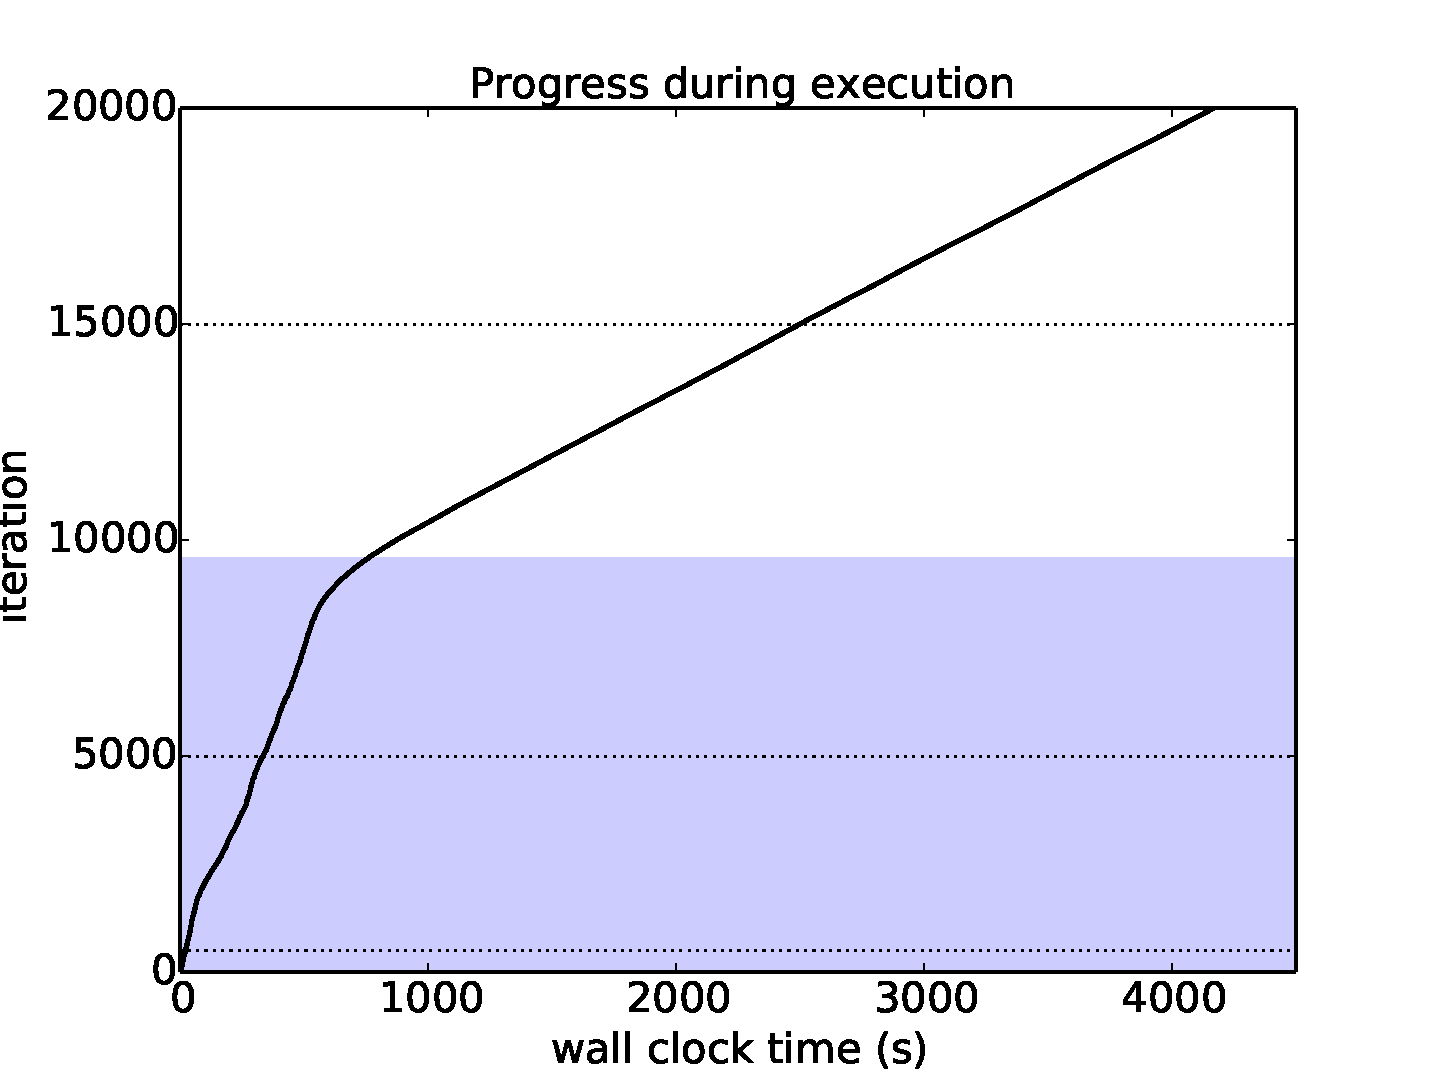
\includegraphics[width=0.65\textwidth]{\fdir/inverted.pdf}
\end{center}
\caption{Progress as a function of wall clock time, in seconds, for the mixture
of Gaussians problem with 64 workers.
This experiment is the same as the second in Figure~\ref{fig:mixture}.
The dotted horizontal lines are at 500, 5000 and 15000 iterations
and correspond to the three iteration counts highlighted in
Figures~\ref{fig:stacked-worker} and~\ref{fig:stacked-master}.
We plot the progress out to 20000 iterations; the behavior remains stable for
the remainder of the experiment, out to 50000 iterations.}
\label{fig:progress}
\end{figure}



Over the course of execution, we measured the total time all worker cores
spent on five different tasks: generating useful proposals, wasted proposals,
useful target evaluation, wasted target evaluation
and waiting for a work assignment from the master.
Figure~\ref{fig:stacked-worker} summarizes these results by plotting the
fraction of time spent performing useful work (blue),
wasted work (light gray, hatched) and waiting (light gray, solid).
The fraction of time spent on useful work corresponds to efficiency
and decreases as execution progresses.
%
Figure~\ref{fig:stacked-master} shows utilization on the master,
divided into time spent acting in response to worker messages (blue)
and  time spent waiting for worker messages (light gray).
Utilization on the master is stable for the entire execution;
the master is active for less than~5\% of the time.

\begin{figure}[t!]
\begin{center}
\includegraphics[width=0.65\textwidth]{\fdir/stacked-worker.pdf}
\end{center}
\vspace{-0.1in}
\caption{Cumulative fraction of time an average worker (64 total) spent performing
useful (blue) or wasted (light gray, hatched) work, and waiting for work (light gray),
normalized with respect to wall clock time, at three representative iteration counts.
These measurements do not include the initial start-up time before each worker
sends its first \WANTWORK message.
After 500 iterations, this corresponds to less than~5\% of the elapsed time.}
\label{fig:stacked-worker}
\end{figure}
%
\begin{figure}[t!]
\begin{center}
\includegraphics[width=0.65\textwidth]{\fdir/stacked-master.pdf}
\end{center}
\vspace{-0.1in}
\caption{Cumulative fraction of time on master spent acting in response to
messages from~64 workers (blue) and waiting for worker messages (light gray),
normalized with respect to wall clock time, at three representative iteration counts.}
\label{fig:stacked-master}
\end{figure}


Finally, Figure~\ref{fig:allocated-nodes} plots the number of \emph{allocated}
jobtree nodes, \ie nodes explicitly represented in the jobtree stored on the
master, over the course of execution, for~64 workers.
We record this number at the end of each MH iteration.
During burn-in, there are usually hundreds of allocated jobtree nodes,
spanning less than~100 to greater than~500 during this time.
In this phase, the prefetching is more aggressive, leading to irregular but
deeper tree shapes that grow in the number of allocated nodes as predictions change.
The number of allocated nodes decreases, sometimes sharply, whenever portions
of the jobtree are trimmed.
After convergence, the number of allocated nodes stabilizes to a much smaller
range around~64, the number of workers.
Then, the predictions are more or less ambiguous, and our prefetching scheme 
eventually looks more like the na\"ive scheme that densely
allocates nodes starting at the root of the tree.

\begin{figure}[t!]
\centering
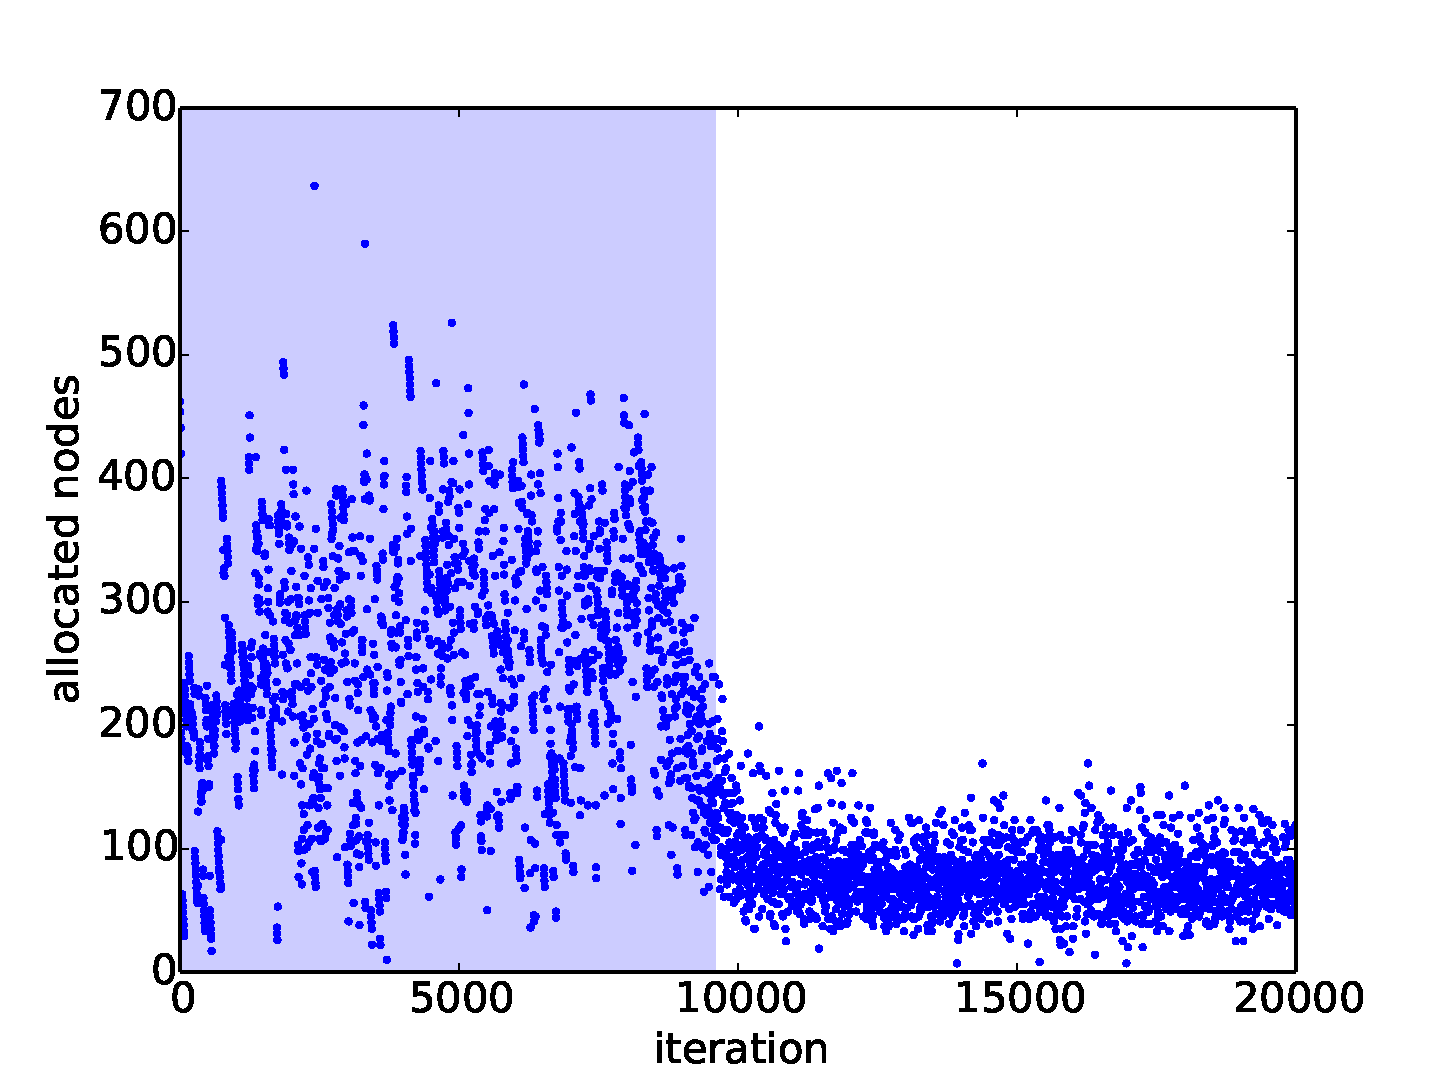
\includegraphics[width=0.65\textwidth]{\fdir/allocated_nodes.pdf}
\caption{The number of allocated jobtree nodes during execution.
Note that the data have been collected upon completion of each iteration
and downsampled by a factor of five.}
\label{fig:allocated-nodes}
\end{figure}


\section{System overheads}
\label{sec:overheads}

%  ** Master CPU not a bottleneck 

% 1000 batches
% master work [ 0.19932927  0.24070103  0.26558971]
% worker wait [ 0.00348117  0.04901537  0.07576223]

% 100 batches
% master work [ 0.03976301  0.05209075  0.04269219]
% worker wait [ 0.02987042  0.00873792  0.00676882]

The primary bottleneck in our implementation is due to the fan-in at the master.
Specifically, our performance is sensitive to the rate at which the master
must process messages from the workers, which scales with both the number of
workers and the number of batches per target function evaluation.
When the master is overwhelmed by messages, the workers end up waiting for work
assignments, which decreases the fraction of time they spend on useful work.
In Section~\ref{sec:measurements}, we summarized utilization on an average
worker and the master, for the mixture of Gaussians problem with 64 workers,
where the likelihood is evaluated in 100 batches.
In this case, the average worker waits for less than~1\% of the time and
the master works for less than~5\% of the time.
Figures~\ref{fig:stacked-worker-wait} and~\ref{fig:stacked-master-work}
illustrate the behavior for the same problem,\footnote{We note that the
initial conditions are different.} where we have decreased the batch 
size by a factor of~10, \ie increased to~1000 batches per likelihood evaluation.
By 10000 iterations, the average worker spends about~10 times longer waiting
(8\%~of the time) and the master spends~5 to~6 times longer working 
(25\%~of the time).

We could address this issue in several ways:  decreasing the number of batches
per target evaluation, eliminating the need for \WANTWORK messages
and dividing the work of the master among multiple cores.
%
In our current design, we use a constant batch size for our updates.
However, this does not reflect information from our error model,
which characterizes predictor uncertainty.
For example, once we are relatively confident that a predictor has converged,
then there isn't much advantage to sending updates in batches.
Alternatively, when the error model indicates high uncertainty, the predictions
carry little weight and not much information is gained until essentially all the
data are evaluated.
With larger batch sizes, we would probably want workers to periodically check
for \ABANDON messages during the evaluation of the batch -- recall that these
can be triggered by any update in the jobtree associated with any ancestral node.
%More generally, our error model can be used to calculate the expected
%information that would be gained by evaluating any amount of additional data.
%
Also currently, the master does not assign work to a worker
until it receives a \WANTWORK message, even though the master knows via
\UPDATE messages when the worker is approaching the end of an assignment
or alternately decides when the worker should stop its current assignment.
Thus, potential improvements could come from two modifications:
the master could eagerly send a \HAVEWORK message to a worker as soon as
it recognizes that the worker is nearing the end of the assignment, and
it could also combine a \HAVEWORK message with an \ABANDON message. 
Note that in the first of these, we wouldn't want the \HAVEWORK messages to be
sent too eagerly, since they would be based on potentially stale predictions.
%
Another strategy for achieving better scalability would be to introduce multiple
submasters, where each is responsible for managing a portion of the jobtree.
%
We leave investigation of all these ideas as future work.


\begin{figure}[t!]
\begin{center}
\includegraphics[width=0.65\textwidth]{\gdir/stacked-worker.pdf}
\end{center}
\vspace{-0.1in}
\caption{Cumulative fraction of time an average worker (64 total) spent performing
useful (blue) or wasted (light gray, hatched) work, and waiting for work
(light gray), normalized with respect to wall clock time.
The number of batches per likelihood evaluation is~10 times greater than in
Figure~\ref{fig:stacked-worker},
and the workers spend about~10 times longer waiting for work.
}
\label{fig:stacked-worker-wait}
\end{figure}
%
\begin{figure}[t!]
\begin{center}
\includegraphics[width=0.65\textwidth]{\gdir/stacked-master.pdf}
\end{center}
\vspace{-0.1in}
\caption{Cumulative fraction of time on master spent acting in response to
messages from~64 workers (blue) and waiting for worker messages (light gray),
normalized with respect to wall clock time.
The number of batches per likelihood evaluation is~10 times greater than in
Figure~\ref{fig:stacked-master},
and utilization of the master is~5 to~6 times higher.}
\label{fig:stacked-master-work}
\end{figure}

\end{document}